\documentclass[10pt]{article}

% Packages
\usepackage[margin=.5in]{geometry}
\usepackage{amsmath,amssymb,amsthm}
\usepackage{enumitem}
\usepackage{hyperref}
\usepackage{xcolor}
\usepackage{import}
\usepackage{xifthen}
\usepackage{pdfpages}
\usepackage{transparent}
\usepackage{listings}
\usepackage{tikz}
\usepackage{physics}
\usepackage{siunitx}
\usepackage{cancel}
  \usetikzlibrary{calc,patterns,arrows.meta,decorations.markings}


\DeclareMathOperator{\Log}{Log}
\DeclareMathOperator{\Arg}{Arg}

\lstset{
    breaklines=true,         % Enable line wrapping
    breakatwhitespace=false, % Wrap lines even if there's no whitespace
    basicstyle=\ttfamily,    % Use monospaced font
    frame=single,            % Add a frame around the code
    columns=fullflexible,    % Better handling of variable-width fonts
}

\newcommand{\incfig}[1]{%
    \def\svgwidth{\columnwidth}
    \import{./Figures/}{#1.pdf_tex}
}
\theoremstyle{definition} % This style uses normal (non-italicized) text
\newtheorem{solution}{Solution}
\newtheorem{proposition}{Proposition}
\newtheorem{problem}{Problem}
\newtheorem{lemma}{Lemma}
\newtheorem{theorem}{Theorem}
\newtheorem{remark}{Remark}
\newtheorem{note}{Note}
\newtheorem{definition}{Definition}
\newtheorem{example}{Example}
\newtheorem{corollary}{Corollary}
\theoremstyle{plain} % Restore the default style for other theorem environments
%

% Theorem-like environments
% Title information
\title{The Big List SP25}
\author{Jerich Lee}
\date{\today}

\begin{document}

\maketitle
\section{PHYS-213}
\begin{problem}
  \textbf{Question 2: Degrees of Freedom}
  
  Suppose we are given a box filled with $6$ moles of an unknown gas with an initial
  temperature of $300~\text{K}$. We add $1.45\times10^{4}\,\text{J}$ of heat to the gas
  and find that the final temperature of the gas is $383~\text{K}$.
  
  \medskip
  Assuming equipartition applies, how many degrees of freedom are active in the gas?
  
  \begin{enumerate}
    \item[(a)] $6$
    \item[(b)] $7$
    \item[(c)] $5$
    \item[(d)] $3$
    \item[(e)] $15$
  \end{enumerate}
  \end{problem}
  %--------------------------------------------------------------------
% Problem: Boltzmann probabilities in a three-state system
%--------------------------------------------------------------------
\begin{problem}
  A three-state system is in an environment at temperature
  $605\,\text{K}$.  
  The energy of state~1 is $E_{1}=3.2\times10^{-20}\,\text{J}$ and the
  energy of state~3 is $E_{3}=4.8\times10^{-20}\,\text{J}$.  
  The energy of state~2 equals that of state~1, so $E_{2}=E_{1}$, while
  state~3 has the largest energy ($E_{3}>E_{2}=E_{1}$).
  
  \medskip
  What is the probability that the system is in state~3?
  
  \begin{enumerate}
    \item[(a)] $0.147$
    \item[(b)] $0.128$
    \item[(c)] $0.333$
    \item[(d)] $0.5$
    \item[(e)] $0.0685$
  \end{enumerate}
  \end{problem}
  
  %--------------------------------------------------------------------
  % Problem: Equal probabilities for two states
  %--------------------------------------------------------------------
  \begin{problem}
  What would make the probability of the system being in state~1 equal to
  the probability of state~3?
  
  \begin{enumerate}
    \item[(a)] $T = 0$
    \item[(b)] $T \to \infty$
    \item[(c)] $E_{2} > E_{1}$
  \end{enumerate}
  \end{problem}
  \begin{problem}
    Consider the graph pictured here, which represents the equilibrium concentration \(p\) of impurity atoms (labeled \(1\text{–}5\)) in silicon.  
    Assume the atoms form an ideal solution obeying
    \[
       p \;=\; p_{0}\exp\!\Bigl(-\tfrac{\Delta}{kT}\Bigr).
    \]
    
    Of the following materials, which has the \emph{largest} energetic cost \(\Delta\) for inserting an atom into the silicon lattice?
    
    \[
    \begin{array}{c|cc|cc}
    \text{Material} & x_{1} & y_{1} & x_{2} & y_{2}\\ \hline
    1 & 0.5 & 28.74 & 2 & 25.67\\
    2 & 0.5 & 27.11 & 2 & 22.58\\
    3 & 0.5 & 20.71 & 2 & 14.71\\
    4 & 0.5 & 29.89 & 2 & 29.74\\
    5 & 0.5 & 21.73 & 2 & 20.11
    \end{array}
    \]
    
    \begin{enumerate}
      \item[(a)] Material 4
      \item[(b)] Material 2
      \item[(c)] Material 5
      \item[(d)] Material 3
      \item[(e)] Material 1
    \end{enumerate}
    \end{problem}
    \begin{problem}
      Consider the heat engine shown below, operated in contact with a hot thermal reservoir at temperature \(T_H = 100\,^{\circ}\text{C}\) and a cold thermal reservoir at temperature \(T_C\).
      
      \medskip
      Suppose that the engine must generate \(600\ \text{W}\) of useful work while drawing \(1000\ \text{W}\) of heat from the hot thermal reservoir.  What is the \emph{maximum} temperature that the cold reservoir could have?
      
      \smallskip
      \textit{Note the units in the answers.}
      
      \begin{enumerate}
        \item[(a)] \(60\,^{\circ}\text{C}\)
        \item[(b)] \(149\,^{\circ}\text{C}\)
        \item[(c)] \(40\,^{\circ}\text{C}\)
        \item[(d)] \(-49.3\,^{\circ}\text{C}\)
        \item[(e)] \(-124\,^{\circ}\text{C}\)
      \end{enumerate}
      \end{problem}
      \begin{problem}
        \textbf{Question 9: Boiling}
        
        Use the fact that
        \[
          d\mu_X \;=\; \frac{V_X}{N_X}\,dp \;-\; \frac{S_X}{N_X}\,dT
          \]
        to determine how much the pressure must change in order to \emph{lower}
        the boiling point of water by a small amount of \(0.13\;\text{K}\).
        
        You may assume that the entropy and density of both liquid and gas are
        roughly constant for these small changes.  You may also assume that the
        molar volume of liquid water is negligible compared with that of water
        vapor and that water vapor behaves as an ideal gas.
        
        \medskip
        \textit{Useful constants}
        \begin{itemize}
          \item Atmospheric pressure: \(1.01300\times10^{5}\;\text{Pa}\)
          \item Boiling point of water at atmospheric pressure: \(373.15\;\text{K}\)
          \item Entropy difference (liquid \(\rightarrow\) gas) per kilogram:
                \(6.05\times10^{3}\;\text{J\,kg}^{-1}\text{K}^{-1}\)
          \item Molecular weight of water: \(0.018\;\text{kg\,mol}^{-1}\)
        \end{itemize}
        
        \medskip
        How much must the pressure change?
        
        \begin{enumerate}
          \item[(a)] \(0.00\times10^{0}\;\text{Pa}\)
          \item[(b)] \(1.72\times10^{6}\;\text{Pa}\)
          \item[(c)] \(2.28\times10^{26}\;\text{Pa}\)
          \item[(d)] $1.56e28 \text{Pa} $ 
          \item[(d)] \(4.50\times10^{2}\;\text{Pa}\)
        \end{enumerate}
        \end{problem}
        \begin{problem}
          \textbf{Question 15: Entropy of Coins}
          
          You toss a fair coin (equal probability of heads and tails) \(16\) times and record the total number of heads.  
          Which value for the total number of heads has the \emph{lowest} entropy?
          
          \begin{enumerate}
            \item[(a)] \(12\)
            \item[(b)] \(4\)
            \item[(c)] \(14\)
            \item[(d)] \(3\)
            \item[(e)] \(8\)
          \end{enumerate}
          \end{problem}
          \begin{problem}
            \textbf{Question 15: Cold Stone}
            
            Suppose that we have a block of metal with \emph{constant but unknown} heat
            capacity.  
            The block is initially at the temperature of liquid nitrogen
            \(\bigl(T = 77\,\text{K}\bigr)\).
            We use this cold metal block to power a heat engine, taking the surrounding
            air at room temperature \(\bigl(T_{1}=294\,\text{K}\bigr)\) as the hot thermal
            reservoir, and we observe that \emph{at most}
            \(80\,\text{kJ}\) of useful work can be extracted from the engine.
            
            \medskip
            What is the heat capacity of the block?
            
            \begin{enumerate}
              \item[(a)] \(4.6\times10^{2}\;\text{J\,K}^{-1}\)
              \item[(b)] \(2.5\times10^{2}\;\text{J\,K}^{-1}\)
              \item[(c)] \(8.0\times10^{2}\;\text{J\,K}^{-1}\)
              \item[(d)] \(-2.0\times10^{2}\;\text{J\,K}^{-1}\)
              \item[(e)] \(-3.7\times10^{2}\;\text{J\,K}^{-1}\)
            \end{enumerate}
            \end{problem}
            \begin{problem}
              A three‐state system is in an environment at temperature \(605\;\text{K}\).
              The energy of state 1 is \(E_{1}=3.2\times10^{-20}\;\text{J}\) and the energy of
              state 3 is \(E_{3}=4.8\times10^{-20}\;\text{J}\).
              State 2 has the same energy as state 1, i.e.\ \(E_{2}=E_{1}\), while state 3
              has the largest energy \((E_{3}>E_{2}=E_{1})\).
              
              \medskip
              Answer the following three questions about this system:
              
              \begin{enumerate}
                \item \textbf{Probability of state 3.}\;
                      What is the probability that the system is in state 3?
                      \begin{enumerate}
                        \item[(a)] \(0.333\)
                        \item[(b)] \(0.147\)
                        \item[(c)] \(0.128\)
                        \item[(d)] \(0.0685\)
                        \item[(e)] \(0.5\)
                      \end{enumerate}
              
                \item \textbf{Equal probabilities for states 1 and 3.}\;
                      Which condition would make the probability of the system being in
                      state 1 equal to the probability of being in state 3?
                      \begin{enumerate}
                        \item[(a)] \(E_{2} > E_{1}\)
                        \item[(b)] \(T \to \infty\)
                        \item[(c)] \(T = 0\)
                      \end{enumerate}
              
                \item \textbf{Zero entropy.}\;
                      Which condition would lead to the entropy of the system being zero?
                      \begin{enumerate}
                        \item[(a)] \(T = 0\)
                        \item[(b)] \(T \to \infty\)
                        \item[(c)] \(E_{2} > E_{1}\)
                      \end{enumerate}
              \end{enumerate}
              \end{problem}
              \begin{problem}
                \textbf{Question 6: Bath}
                
                A system has states with energies \(E_{1} = 0.4\;\text{eV}\) and \(E_{2} = 0.6\;\text{eV}\).
                There is only a single state with energy \(E_{1}\), but there are two states with energy \(E_{2}\).
                
                \medskip
                What is the average energy of the system as the temperature \(T\) approaches infinity?
                
                \begin{enumerate}
                  \item[(a)] \(0.400\;\text{eV}\)
                  \item[(b)] \(0.600\;\text{eV}\)
                  \item[(c)] \(0.500\;\text{eV}\)
                  \item[(d)] \(0.533\;\text{eV}\)
                  \item[(e)] \(0.467\;\text{eV}\)
                \end{enumerate}
                \end{problem}
                \begin{problem}
                  \textbf{Question 16: Gas}
                  
                  Suppose a diatomic ideal gas expands under \emph{constant temperature}.
                  The initial and final pressures are
                  \(P_i = 700\ \text{Pa}\) and \(P_f = 850\ \text{Pa}\), respectively.
                  The temperature is fixed at \(T = 600\ \text{K}\) and the number of
                  molecules at \(N = 7\times10^{23}\).
                  What is the change in Gibbs free energy for this process?
                  
                  You may assume that only translational and rotational degrees of
                  freedom are active.
                  
                  \begin{enumerate}
                    \item[(a)] \(6.753\times10^{2}\ \text{J}\)
                    \item[(b)] \(1.876\times10^{3}\ \text{J}\)
                    \item[(c)] \(1.125\times10^{3}\ \text{J}\)
                    \item[(d)] \(2.378\times10^{3}\ \text{J}\)
                    \item[(e)] \(9.000\times10^{0}\ \text{J}\)
                  \end{enumerate}
                  \end{problem}
                  \begin{problem}
                    \textbf{(D) Vapor Pressure of Water}
                    
                    Now let us make a crude picture of how the vapor pressure of water varies
                    with temperature \(T\).
                    Suppose the vapor is a collection of molecules in states whose energies
                    exceed those of the liquid by an amount \(\Delta E\), because each molecule
                    loses some energy when it sticks to its neighbors in the liquid.
                    Consequently, the concentration \(n\) of molecules in the vapor will fall
                    off as \(\exp(-\Delta E/kT)\) compared with the nearly fixed concentration
                    of molecules in the (essentially incompressible) liquid.
                    Because \(p = nkT\), the vapor pressure \(p\) is proportional to
                    \(T\,\exp(-\Delta E/kT)\); it therefore changes rapidly with \(T\) owing to
                    the Boltzmann factor.
                    
                    Keeping better track of the way the number of states available in the
                    liquid and gas vary with \(T\) instead gives the
                    \emph{Clausius--Clapeyron relation}
                    \[
                       p \;=\; p_{0}\,\exp\!\Bigl(-\tfrac{L}{kT}\Bigr),
                    \]
                    where \(L\)---the latent heat \emph{per molecule}---is very nearly the same
                    \(\Delta E\) introduced above.
                    Thus the exponential dependence of the vapor pressure on \(1/T\) is
                    ultimately an expression of the Boltzmann factor.
                    
                    \begin{enumerate}
                      \item[(i)] Sketch the expected curve for \(\ln p\) versus \(1/T\)
                                 (\emph{not} versus \(T\)).
                      \item[(ii)] Explain how the slope of this curve can be used to determine
                                  the value of \(L\).
                    \end{enumerate}
                    
                    \bigskip
                    \textbf{(E) Pressure Cooker}
                    
                    Water boils at \(373\;\text{K}\) (\(100^{\circ}\text{C}\)) when the
                    pressure is \(1\;\text{atm}\).
                    Assuming the Clausius--Clapeyron relation above holds, and using the value
                    of \(L\) you obtained earlier, calculate the boiling temperature of water
                    inside a pressure cooker that operates at \(2\;\text{atm}\).
                    \end{problem}
                    \begin{problem}
                      \textbf{Question 12: Chemical Potential}
                      
                      Suppose that at a pressure of \(1\;\text{atm}\) and a temperature of
                      \(300\;\text{K}\), a given material can exist in two phases:
                      liquid \((L)\) and solid \((S)\).
                      We start the system with
                      \[
                         N_{L}=5\;\text{mol}, \qquad
                         N_{S}=2\;\text{mol}.
                      \]
                      
                      For these values of pressure and temperature, the chemical potentials are
                      \[
                         \mu_{L}=5\times10^{-20}\,\text{J}, \qquad
                         \mu_{S}=9\times10^{-21}\,\text{J}.
                      \]
                      
                      \medskip
                      What is the equilibrium value of \(N_{S}\)?
                      
                      \begin{enumerate}
                        \item[(a)] \(2\) moles
                        \item[(b)] \(5\) moles
                        \item[(c)] \(7\) moles
                        \item[(d)] \(0\) moles
                        \item[(e)] \(1.49\) moles
                      \end{enumerate}
                      \end{problem}
                      \begin{problem}
                        A \emph{heat pump} is used to maintain the temperature of a house (the hot
                        reservoir) at \(T_{h}=21^{\circ}\mathrm{C}\) while discharging heat to the
                        outdoors (the cold reservoir) at \(T_{c}=-11^{\circ}\mathrm{C}\).
                        During an Urbana winter night the house loses heat to the outside at a
                        rate of \(Q_{\text{leak}} = 26\;\text{kW}\).
                        
                        Assuming the pump operates reversibly (i.e., with the Carnot coefficient
                        of performance), what is the \textbf{minimum} electric power \(W\)
                        required to supply the heat \(Q_{h}=Q_{\text{leak}}\) and keep the house
                        at \(T_{h}\)?
                        
                        \begin{enumerate}
                          \item[(a)] \(1.4\;\text{kW}\)
                          \item[(b)] \(2.8\;\text{kW}\)  % correct
                          \item[(c)] \(4.3\;\text{kW}\)
                          \item[(d)] \(9.3\;\text{kW}\)
                          \item[(e)] \(26\;\text{kW}\)
                        \end{enumerate}
                        \end{problem}
                        \begin{problem}
                          \textbf{Question 8: Heat Capacity}
                          
                          What is the heat capacity of \(4\;\text{kg}\) of solid germanium at room
                          temperature?  Assume that equipartition holds.
                          
                          \begin{enumerate}
                            \item[(a)] \(9.38\times10^{1}\;\text{J\,K}^{-1}\)
                            \item[(b)] \(1.37\times10^{0}\;\text{J\,K}^{-1}\)
                            \item[(c)] \(6.83\times10^{2}\;\text{J\,K}^{-1}\)
                            \item[(d)] \(1.37\times10^{3}\;\text{J\,K}^{-1}\)
                            \item[(e)] \(4.99\times10^{1}\;\text{J\,K}^{-1}\)
                          \end{enumerate}
                          \end{problem}
                          \begin{problem}
                            Consider a large centrifuge that spins very quickly so that the
                            centrifugal acceleration in the tube is \(3g\) directed toward the bottom
                            of the tube, where \(g = 9.8\;\text{m\,s}^{-2}\).
                            Each tube is \(0.30\;\text{m}\) long.
                            Inside the tube is a gas mixture of
                            
                            \[
                               \text{hemoglobin molecules: } m_{\mathrm{Hb}} = 1.07\times10^{-22}\,\text{kg},
                               \qquad
                               \text{N}_{2}\text{ molecules: } m_{\mathrm{N_2}} = 4.65\times10^{-26}\,\text{kg}.
                            \]
                            
                            The tube is allowed to reach thermal equilibrium with the surroundings at
                            \(T = 312\;\text{K}\).
                            
                            \medskip
                            \textbf{Part 1}
                            
                            Suppose the average number of hemoglobin molecules found at height
                            \(h_{1}=0.03\;\text{m}\) is \(N_{1}=2.0\times10^{4}\).
                            What is the average number of hemoglobin molecules located at
                            \(h_{2}=0.20\;\text{m}\)?
                            
                            \begin{enumerate}
                              \item[(a)] \(2.86\times10^{3}\)
                              \item[(b)] \(1.40\times10^{5}\)
                              \item[(c)] \(1.82\times10^{3}\)
                              \item[(d)] \(1.33\times10^{4}\)
                              \item[(e)] \(1.77\times10^{4}\)
                            \end{enumerate}
                            
                            \bigskip
                            \textbf{Part 2}
                            
                            Which type of molecule will be most prevalent at the \emph{top} of the
                            tube once equilibrium is reached?
                            
                            \begin{enumerate}
                              \item[(a)] \(\mathrm{N_2}\)
                              \item[(b)] hemoglobin
                              \item[(c)] They will be in equal proportions throughout the tube.
                            \end{enumerate}
                            \end{problem}
                            \begin{problem}
                              \textbf{Question 7: Equipartition in a Solid}
                              
                              A quantity of \(700\;\text{J}\) of heat is applied to \(1\;\text{kg}\) of an unknown solid, and its temperature is observed to rise by \(6^{\circ}\text{C}\).
                              
                              Assuming equipartition holds, what is the molar mass of the solid?
                              
                              \begin{enumerate}
                                \item[(a)] \(0.00857\;\text{g\,mol}^{-1}\)
                                \item[(b)] \(107\;\text{g\,mol}^{-1}\)
                                \item[(c)] \(9.95\;\text{g\,mol}^{-1}\)
                                \item[(d)] \(71.3\;\text{g\,mol}^{-1}\)
                                \item[(e)] \(214\;\text{g\,mol}^{-1}\)
                              \end{enumerate}
                              \end{problem}
                              \begin{problem}
                                Nine moles of a monatomic ideal gas are heated from an initial temperature of
                                \(250\;\text{K}\) to a final temperature of \(280\;\text{K}\) by adding
                                \(3523\;\text{J}\) of heat.  How much work is done \emph{by the gas}
                                during this expansion?
                                
                                (Assume only translational degrees of freedom are active.)
                                
                                \begin{enumerate}
                                  \item[(a)] \(-1.56\times10^{2}\;\text{J}\)
                                  \item[(b)] \(-2.24\times10^{3}\;\text{J}\)
                                  \item[(c)] \(2.24\times10^{3}\;\text{J}\)
                                  \item[(d)] \(0\;\text{J}\)
                                  \item[(e)] \(1.56\times10^{2}\;\text{J}\)
                                \end{enumerate}
                                \end{problem}
                                \begin{problem}
                                  \textbf{Question 7: Chemical Equilibrium}
                                  
                                  Suppose we place an unknown material in a cylinder of fixed volume at fixed
                                  temperature.  Under these conditions the material may exist either as a
                                  liquid \((\ell)\) or as a gas \((g)\).
                                  Thermodynamic analysis of the free energy shows that
                                  
                                  \[
                                     \mu_{g}-\mu_{\ell} \;=\; \Delta + kT\,
                                     \ln\!\Bigl(\frac{N_{g}}{N_{\ell}}\Bigr),
                                  \]
                                  
                                  where \(\mu_{g}\) and \(\mu_{\ell}\) are the chemical potentials of the gas
                                  and liquid, \(N_{g}\) and \(N_{\ell}\) are the numbers of molecules in each
                                  phase, \(k\) is Boltzmann’s constant, and \(\Delta=0.394\;\text{eV}\).
                                  
                                  \medskip
                                  When the liquid and gas reach equilibrium, the ratio
                                  \(N_{g}/N_{\ell}\) is measured to be \(0.541\).
                                  What is the temperature \(T\) of the system?
                                  
                                  \begin{enumerate}
                                    \item[(a)] \(7.28\;\text{K}\)
                                    \item[(b)] \(8.34\times10^{-4}\;\text{K}\)
                                    \item[(c)] \(10.0\;\text{K}\)
                                    \item[(d)] \(7.44\times10^{3}\;\text{K}\)  % correct
                                    \item[(e)] \(8.45\times10^{3}\;\text{K}\)
                                  \end{enumerate}
                                  \end{problem}
                                  \begin{problem}
                                    Consider a Carnot (i.e.\ reversible) engine operating between a hot
                                    reservoir at temperature \(T_{h}\) and a cold reservoir at
                                    temperature \(T_{c}\).
                                    The Carnot efficiency of this engine is \(\varepsilon = 30\%\), and it
                                    performs \(120\ \text{J}\) of work during each cycle.
                                    
                                    \medskip
                                    What is the ratio \(T_{c}/T_{h}\) for this engine?
                                    
                                    \begin{enumerate}
                                      \item[(a)] \(3.33\)
                                      \item[(b)] \(0.30\)
                                      \item[(c)] \(1.00\)
                                      \item[(d)] \(1.43\)
                                      \item[(e)] \(0.70\)
                                    \end{enumerate}
                                    \end{problem}
                                    \begin{problem}
                                      \textbf{Question 6: Ideal Gases}
                                      
                                      Consider a sealed box of fixed volume that initially contains an \emph{equal}
                                      number of helium (\(\mathrm{He}\)) and nitrogen (\(\mathrm{N_{2}}\)) molecules
                                      in equilibrium at temperature \(T_{0}=300\;\text{K}\) and pressure
                                      \(P_{0}=1\;\text{atm}\).
                                      
                                      \medskip
                                      Suppose the box is cooled to \(T_{1}=30\;\text{K}\).
                                      At this temperature the helium remains in the gaseous phase, whereas the
                                      nitrogen solidifies and sticks permanently to the walls of the box.
                                      The volume of the box and the number of helium molecules therefore remain
                                      unchanged.
                                      
                                      \smallskip
                                      What is the pressure inside the box after cooling?
                                      
                                      \begin{enumerate}
                                        \item[(a)] \(1\;\text{atm}\)
                                        \item[(b)] \(10\;\text{atm}\)
                                        \item[(c)] \(0.05\;\text{atm}\)
                                        \item[(d)] \(0.1\;\text{atm}\)
                                        \item[(e)] \(0.5\;\text{atm}\)
                                      \end{enumerate}
                                      \end{problem}
                                      \begin{problem}
                                        \textbf{Question 10: Heat Capacity}
                                        
                                        Consider a non-ideal monatomic gas whose equation of state is
                                        \[
                                           \bigl(P + a\bigr)V \;=\; nRT,
                                           \qquad a = 0.10\;\text{atm}.
                                        \]
                                        Assuming the internal energy of the gas is well described by equipartition,
                                        what is \(C_{p} - C_{v}\) for \(7\) moles of the gas at a pressure of
                                        \(3\;\text{atm}\) and a temperature of \(403\;\text{K}\)?
                                        
                                        \begin{enumerate}
                                          \item[(a)] \(5.82\times10^{1}\;\text{J\,K}^{-1}\)
                                          \item[(b)] \(-5.63\times10^{1}\;\text{J\,K}^{-1}\)
                                          \item[(c)] \(-5.82\times10^{1}\;\text{J\,K}^{-1}\)
                                          \item[(d)] \(1.88\times10^{1}\;\text{J\,K}^{-1}\)
                                          \item[(e)] \(6.53\times10^{1}\;\text{J\,K}^{-1}\)
                                        \end{enumerate}
                                        \end{problem}
                                        \begin{problem}
                                          Consider the schematic phase diagram shown below.  
                                          The three regions correspond to distinct phases labeled
                                          \(\text{Phase I}\), \(\text{Phase II}\), and \(\text{Phase III}\).
                                          The thick lines denote the coexistence curves, which meet at a single
                                          triple point.
                                          
                                          \begin{center}
                                          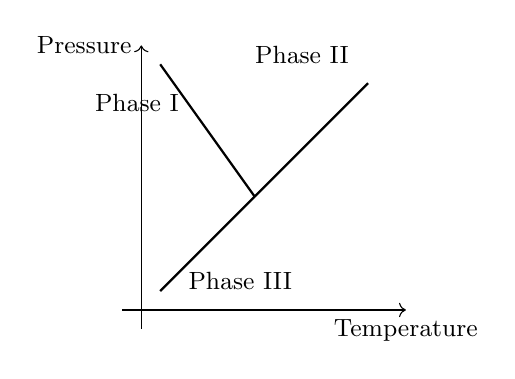
\begin{tikzpicture}[scale=2.4, every node/.style={font=\small}]
                                            % axes
                                            \draw[->] (-0.1,0) -- (1.4,0) node[below] {Temperature};
                                            \draw[->] (0,-0.1) -- (0,1.4) node[left] {Pressure};
                                            % coexistence lines
                                            \coordinate (O) at (0.6,0.6); % triple point
                                            \draw[thick] (O) -- (0.1,1.3);            % I–II
                                            \draw[thick] (O) -- (1.2,1.2);            % II–III
                                            \draw[thick] (O) -- (0.1,0.1);            % I–III
                                            % phase labels
                                            \node[anchor=south east] at (0.25,1.0) {Phase~I};
                                            \node[anchor=south]      at (0.85,1.25) {Phase~II};
                                            \node[anchor=north east] at (0.85,0.25) {Phase~III};
                                          \end{tikzpicture}
                                          \end{center}
                                          
                                          Near any coexistence line, the chemical potentials of the two phases are
                                          equal, and small changes satisfy
                                          \[
                                            d\mu \;=\; \frac{V}{N}\,dp \;-\; \frac{S}{N}\,dT.
                                          \]
                                          
                                          \medskip
                                          \textbf{Which statement must be true about the phases adjacent to the
                                          coexistence curves?}
                                          
                                          \begin{enumerate}
                                            \item[(a)] Phase~II is \emph{denser} than Phase~I.
                                            \item[(b)] Phase~I has \emph{more entropy per particle} than Phase~II.
                                            \item[(c)] Phase~I has \emph{more entropy per particle} than Phase~III.
                                            \item[(d)] Phase~II has \emph{more entropy per particle} than Phase~III.
                                            \item[(e)] Phase~III is \emph{denser} than Phase~I.
                                          \end{enumerate}
                                          \end{problem}
                                          \begin{problem}
                                            \textbf{Question 7: Chemical Equilibrium}
                                            
                                            Suppose an unknown material is confined in a cylinder of fixed volume at fixed
                                            temperature; the material may exist either as a liquid \((\ell)\) or a gas
                                            \((g)\).
                                            An analysis of the Helmholtz free energy shows that the chemical potentials of
                                            the two phases obey
                                            \[
                                               \mu_{g}-\mu_{\ell}
                                                 \;=\;
                                                 \Delta
                                                 + kT\,\ln\!\Bigl(\tfrac{N_{g}}{N_{\ell}}\Bigr),
                                            \]
                                            where \(N_{g}\) and \(N_{\ell}\) are the numbers of molecules in the gas and
                                            liquid, respectively, \(k\) is Boltzmann’s constant, and
                                            \(\Delta = 0.394\;\text{eV}\).
                                            
                                            \medskip
                                            When the liquid and gas reach equilibrium, the ratio \(N_{g}/N_{\ell}\) is
                                            measured to be \(0.541\).
                                            What is the temperature \(T\) of the system?
                                            
                                            \begin{enumerate}
                                              \item[(a)] \(7.28\;\text{K}\)
                                              \item[(b)] \(8.34\times10^{-4}\;\text{K}\)
                                              \item[(c)] \(0.00\;\text{K}\)
                                              \item[(d)] \(7.44\times10^{3}\;\text{K}\)
                                              \item[(e)] \(8.45\times10^{3}\;\text{K}\)
                                            \end{enumerate}
                                            \end{problem}
                                            \begin{problem}
                                              \textbf{Question 3: Gas}
                                              
                                              How many ideal–gas molecules are contained in a \(1.7\;\text{L}\) tank at a
                                              pressure of \(10\;\text{atm}\) and a temperature of \(303\;\text{K}\)?
                                              
                                              \begin{enumerate}
                                                \item[(a)] \(8.81\times10^{23}\) molecules
                                                \item[(b)] \(1.43\times10^{21}\) molecules
                                                \item[(c)] \(2.55\times10^{26}\) molecules
                                                \item[(d)] \(4.12\times10^{23}\) molecules  % correct
                                                \item[(e)] \(2.77\times10^{21}\) molecules
                                              \end{enumerate}
                                              \end{problem}
                                              \begin{problem}
                                                \textbf{Question 3: Isobaric and Isochoric}
                                                
                                                A gas at \(P = 4.00339\times10^{5}\,\text{Pa}\) is contained in a cylinder
                                                with a movable piston.  
                                                During an \emph{isobaric} (constant–pressure) expansion the gas is heated
                                                and its volume increases from \(0.25\;\text{m}^{3}\) to \(0.55\;\text{m}^{3}\).
                                                
                                                \medskip
                                                \textbf{(A) Work Done}
                                                
                                                What is the work done \emph{by the gas} during this expansion?
                                                
                                                \begin{enumerate}
                                                  \item[(a)] \(60.1\;\text{kJ}\)
                                                  \item[(b)] \(-60.1\;\text{kJ}\)
                                                  \item[(c)] \(120.1\;\text{kJ}\)
                                                  \item[(d)] \(-120.1\;\text{kJ}\)
                                                  \item[(e)] \(240.2\;\text{kJ}\)
                                                \end{enumerate}
                                                
                                                \bigskip
                                                \textbf{(B) Isochoric Heating}
                                                
                                                Next the piston is fixed so the gas remains at constant volume
                                                (\emph{isochoric} process) while it is heated.
                                                
                                                Which of the following statements is true for this isochoric process?
                                                
                                                \begin{enumerate}
                                                  \item[(a)] The area under the \(P\)-versus-\(V\) curve will be the same as for the isobaric case.
                                                  \item[(b)] The pressure inside the cylinder will decrease.
                                                  \item[(c)] The internal energy of the gas will be constant.
                                                  \item[(d)] No work is done on the gas.
                                                \end{enumerate}
                                                \end{problem}
                                                \begin{problem}
                                                  \textbf{Thermodynamic Cycle on a $P$–$V$ Diagram}
                                                  
                                                  Below is the $P$–$V$ diagram for a four–step thermodynamic cycle (all
                                                  processes are straight-line segments).  
                                                  The working fluid is $2$ moles of an ideal \emph{diatomic} gas
                                                  (active degrees of freedom: translation and rotation).
                                                  
                                                  \medskip
                                                  \begin{center}
                                                  \begin{tabular}{c|c|c}
                                                  \textbf{Point} & \textbf{Volume $V$ (m$^{3}$)} & \textbf{Pressure $P$ (Pa)}\\\hline
                                                  1 & 1.2 & 1027\\
                                                  2 & 1.4 & 1460\\
                                                  3 & 1.4 & 1534\\
                                                  4 & 1.2 & 1156
                                                  \end{tabular}
                                                  \end{center}
                                                  
                                                  \medskip
                                                  Answer the following questions.  (Use the sign convention that \emph{work
                                                  done \underline{by} the gas} is positive and \emph{heat added to the gas}
                                                  is positive.)
                                                  
                                                  \begin{enumerate}
                                                    \item \textbf{Work during segment $1 \rightarrow 2$}\,:  
                                                          How much work is done by the gas?
                                                          \begin{enumerate}
                                                            \item[(a)] $0.00\times10^{0}\,\text{J}$
                                                            \item[(b)] $2.49\times10^{2}\,\text{J}$
                                                            \item[(c)] $-3.57\times10^{2}\,\text{J}$
                                                            \item[(d)] $2.92\times10^{2}\,\text{J}$
                                                            \item[(e)] $1.19\times10^{2}\,\text{J}$
                                                          \end{enumerate}
                                                  
                                                    \item \textbf{Heat during segment $4 \rightarrow 1$}\,:  
                                                          How much heat is \emph{added} to the gas?
                                                          \begin{enumerate}
                                                            \item[(a)] $3.87\times10^{2}\,\text{J}$
                                                            \item[(b)] $-1.55\times10^{2}\,\text{J}$
                                                            \item[(c)] $-3.87\times10^{2}\,\text{J}$
                                                            \item[(d)] $1.55\times10^{2}\,\text{J}$
                                                            \item[(e)] $0.00\times10^{0}\,\text{J}$
                                                          \end{enumerate}
                                                  \end{enumerate}
                                                  \end{problem}
                                                  \begin{problem}
                                                    \textbf{Question 5: Simple Harmonic Oscillator v2}
                                                    
                                                    Consider a system of three quantum harmonic oscillators.  
                                                    The system is isolated from the environment with a total of \(7\) quanta of energy.  
                                                    One oscillator has such a high frequency that it always possesses zero quanta,  
                                                    while the other two oscillators have identical frequencies and share the \(7\) quanta.
                                                    
                                                    \medskip
                                                    What is the entropy of the system?
                                                    
                                                    \begin{enumerate}
                                                      \item[(a)] \(2.87\times10^{-23}\ \text{J\,K}^{-1}\)
                                                      \item[(b)] \(7\ \text{J\,K}^{-1}\)
                                                      \item[(c)] \(8\ \text{J\,K}^{-1}\)
                                                      \item[(d)] \(3.64\times10^{-23}\ \text{J\,K}^{-1}\)
                                                      \item[(e)] \(2.69\times10^{-23}\ \text{J\,K}^{-1}\)
                                                    \end{enumerate}
                                                    \end{problem}
                                                    \begin{problem}
                                                      Suppose that during one cycle, a heat engine draws
                                                      \(1200\;\text{J}\) of heat from a hot thermal reservoir.
                                                      What is the \emph{maximum} amount of work the engine can perform in that cycle?
                                                      
                                                      \begin{enumerate}
                                                        \item[(a)] \(5.40\times10^{2}\,\text{J}\)
                                                        \item[(b)] \(1.08\times10^{3}\,\text{J}\)
                                                        \item[(c)] \(5.16\times10^{2}\,\text{J}\)
                                                        \item[(d)] \(1.20\times10^{3}\,\text{J}\)
                                                        \item[(e)] \(2.29\times10^{0}\,\text{J}\)
                                                      \end{enumerate}
                                                      \end{problem}
                                                      \begin{problem}
                                                        \textbf{Question 9: Entropy and Temperature}
                                                        
                                                        Consider a block whose entropy depends on its internal energy according to
                                                        \[
                                                           S(U)=2\sqrt{aU},
                                                        \]
                                                        where \(a = 124\;\text{J\,K}^{-2}\).
                                                        If the block has \(1123\;\text{J}\) of internal energy, what is its temperature?
                                                        
                                                        \begin{enumerate}
                                                          \item[(a)] \(3.01\times10^{0}\;\text{K}\)
                                                          \item[(b)] \(6.02\times10^{0}\;\text{K}\)
                                                          \item[(c)] \(1.50\times10^{0}\;\text{K}\)
                                                          \item[(d)] \(3.32\times10^{-1}\;\text{K}\)
                                                          \item[(e)] \(9.06\times10^{0}\;\text{K}\)
                                                        \end{enumerate}
                                                        \end{problem}
                                                        \begin{problem}
                                                          \textbf{Question 4: Latent Heat}
                                                          
                                                          You are given an unknown material, \emph{Element X}.  
                                                          At room temperature it is a solid, but when heated to
                                                          \(T = 488\;\text{K}\) at a pressure of \(P = 1.0731\times10^{4}\;\text{Pa}\)
                                                          it melts.  
                                                          The latent heat of fusion is measured to be
                                                          \(L = 121\;\text{J\,g}^{-1}\).
                                                          Mass-spectroscopy gives the molar mass
                                                          \(M = 35\;\text{g\,mol}^{-1}\).
                                                          Upon melting, the specific volume increases by
                                                          \(\Delta v = 0.4\;\text{m}^{3}\,\text{kg}^{-1}\).
                                                          
                                                          \medskip
                                                          What is the difference in entropy per mole between the liquid and solid
                                                          phases, \(\Delta S = S_{\text{liq}} - S_{\text{sol}}\)?
                                                          
                                                          \begin{enumerate}
                                                            \item[(a)] \(4.03\times10^{0}\;\text{J\,mol}^{-1}\text{K}^{-1}\)
                                                            \item[(b)] \(7.08\times10^{-3}\;\text{J\,mol}^{-1}\text{K}^{-1}\)
                                                            \item[(c)] \(1.88\times10^{0}\;\text{J\,mol}^{-1}\text{K}^{-1}\)
                                                            \item[(d)] \(1.47\times10^{2}\;\text{J\,mol}^{-1}\text{K}^{-1}\)
                                                            \item[(e)] \(2.48\times10^{-1}\;\text{J\,mol}^{-1}\text{K}^{-1}\)
                                                          \end{enumerate}
                                                          \end{problem}
                                                          \begin{problem}
                                                            \textbf{Question 8: Diamond Heat Capacity}
                                                            
                                                            Diamond has a heat capacity given by \(C = \alpha T^{3}\) over a wide range
                                                            of temperatures, from \(T = 0\;\text{K}\) up to more than
                                                            \(1500\;\text{K}\).
                                                            
                                                            Suppose you have a piece of diamond at \(T = 0\;\text{K}\) and find that you
                                                            must add \(1000\;\text{J}\) of heat to raise its temperature to
                                                            room temperature \(T = 293\;\text{K}\).
                                                            
                                                            \medskip
                                                            How much heat is required to raise the temperature of the diamond from
                                                            \(T = 0\;\text{K}\) to \(T = 586\;\text{K}\)?
                                                            
                                                            \begin{enumerate}
                                                              \item[(a)] \(4000\;\text{J}\)
                                                              \item[(b)] \(2000\;\text{J}\)
                                                              \item[(c)] \(16000\;\text{J}\)
                                                              \item[(d)] \(1000\;\text{J}\)
                                                              \item[(e)] \(8000\;\text{J}\)
                                                            \end{enumerate}
                                                            \end{problem}
                                                            \begin{problem}
                                                              \textbf{Question 4: Irreversible Engine}
                                                              
                                                              Suppose we have a heat engine that operates between a hot reservoir at
                                                              temperature \(T_{H}=532\;\text{K}\) and a cold reservoir at
                                                              temperature \(T_{C}=346\;\text{K}\).
                                                              In each cycle, the engine absorbs \(155\;\text{J}\) of heat from the hot
                                                              reservoir and converts some of it into work.
                                                              The measured efficiency of the engine is \(\varepsilon = 0.238\).
                                                              
                                                              \medskip
                                                              Assuming the engine itself operates without any internal losses, by how
                                                              much does the \emph{total} entropy increase per cycle?
                                                              
                                                              \begin{enumerate}
                                                                \item[(a)] \(0.650\;\text{J\,K}^{-1}\)
                                                                \item[(b)] \(0.341\;\text{J\,K}^{-1}\)
                                                                \item[(c)] \(0.291\;\text{J\,K}^{-1}\)
                                                                \item[(d)] \(0.00\;\text{J\,K}^{-1}\)
                                                                \item[(e)] \(0.0498\;\text{J\,K}^{-1}\)
                                                              \end{enumerate}
                                                              \end{problem}
                                                              %-----------------------------------------------------
% requires \usepackage{tikz} in the preamble
\begin{problem}

    %--- left column: phase diagram ---------------------------------
    \begin{minipage}[t]{0.44\linewidth}
      \centering
      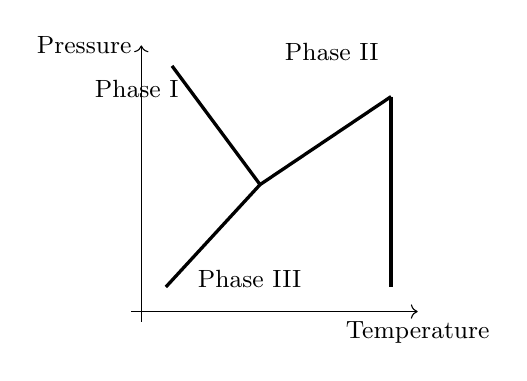
\begin{tikzpicture}[scale=2.6,
                          every node/.style={font=\small}]
        % axes
        \draw[->] (-0.05,0) -- (1.35,0) node[below] {Temperature};
        \draw[->] (0,-0.05) -- (0,1.30) node[left] {Pressure};
        % triple-point
        \coordinate (T) at (0.58,0.62);
        % coexistence curves
        \draw[very thick] (0.12,0.12) -- (T);           % I–III
        \draw[very thick] (T) -- (0.15,1.20);           % I–II
        \draw[very thick] (T) -- (1.22,1.05);           % II–III
        \draw[very thick] (1.22,1.05) -- (1.22,0.12);   % II–III continuation
        % phase labels
        \node[anchor=south east] at (0.23,1.00) {Phase~I};
        \node[anchor=south]      at (0.93,1.18) {Phase~II};
        \node[anchor=north east] at (0.83,0.25) {Phase~III};
      \end{tikzpicture}
    \end{minipage}
    \hfill
    %--- right column: multiple-choice question ----------------------
      Consider the phase diagram shown.
  
      \medskip
      \textbf{Which statement is true about the phases near the phase–
      transition lines between the respective phases?}
      \begin{enumerate}
        \item[(a)] Phase~I has more entropy per particle than Phase~II.
        \item[(b)] Phase~I is denser than Phase~II.
        \item[(c)] Phase~III is denser than Phase~II.
        \item[(d)] Phase~I has more entropy per particle than Phase~III.
        \item[(e)] Phase~III has more entropy per particle than Phase~II.
      \end{enumerate}
  \end{problem}
  %-----------------------------------------------------
\pagebreak                                                        
  \section{MATH-417}
  %------------------------------------------------------------
% requires \usepackage{amsmath} in the preamble
\begin{problem}
  \textbf{Problem 1.}
  Consider the group \((G,\star)\) where \(G=\{-1,0,1\}\) and the group
  operation is defined by
  \[
     a\star b \;=\;
     \begin{cases}
       a+b+1, & \text{if } a+b\le 0,\\[4pt]
       a+b-2, & \text{else.}
     \end{cases}
  \]
  \begin{enumerate}
    \item[(a)] Fill in the multiplication table
          (each row corresponds to a fixed \(a\in G\);
          each column to a fixed \(b\in G\);
          the entry is \(a\star b\)):
  
          \[
          \begin{array}{c|ccc}
            \star & -1 & 0 & 1\\\hline
            -1 & \boxed{\phantom{0}} & \boxed{\phantom{0}} & \boxed{\phantom{0}}\\
             0  & \boxed{\phantom{0}} & \boxed{\phantom{0}} & \boxed{\phantom{0}}\\
             1  & \boxed{\phantom{0}} & \boxed{\phantom{0}} & \boxed{\phantom{0}}
          \end{array}
          \]
  
    \item[(b)] What is the identity element of this group?
    \item[(c)] What is the inverse operation?
    \item[(d)] Verify an example illustrating the associativity of \(G\).
  \end{enumerate}
  \end{problem}
  
  \bigskip
  \begin{problem}
  \textbf{Problem 2.}
  Let \(G\) be a group.
  \begin{enumerate}
    \item[(a)] For \(a,b\in G\), show there exists a \emph{unique} element
              \(x\in G\) such that \(ax=b\).
    \item[(b)] Prove the cancellation law:
              if \(ab=ac\) for some \(a,b,c\in G\), then \(b=c\).
  \end{enumerate}
  \end{problem}
  
  \bigskip
  \begin{problem}
  \textbf{Problem 3.}
  Consider the set
  \(G=\{e^{2\pi i k/5}\mid k=0,1,2,3,4\}\)
  with the usual multiplication \(a\cdot b:=ab\).
  \begin{enumerate}
    \item[(a)] Show that \((G,\cdot)\) is an Abelian group.
    \item[(b)] Determine all subgroups of \(G\).
  \end{enumerate}
  \end{problem}
  
  \bigskip
  \begin{problem}
  \textbf{Problem 4.}
  Let \(d(x,y)\) denote the Euclidean distance between \(x,y\in\mathbb R^{2}\).
  An \emph{isometry} of \(\mathbb R^{2}\) is a bijective map
  \(T:\mathbb R^{2}\to\mathbb R^{2}\) satisfying
  \(d(Tx,Ty)=d(x,y)\) for all \(x,y\in\mathbb R^{2}\).
  \begin{enumerate}
    \item[(a)] Show that the set of all isometries of
              \(\mathbb R^{2}\) forms a group under composition.
    \item[(b)] Conclude that
              \((T_{1}\circ T_{2})(x)=T_{1}\bigl(T_{2}(x)\bigr)\)
              for every \(x\in\mathbb R^{2}\).
  \end{enumerate}
  \end{problem}
  
  \bigskip
  \begin{problem}
  \textbf{Problem 5.}
  For any subgroup \(H\) of \(\bigl(\mathbb Z,+\bigr)\) there exists
  \(k\in\mathbb Z\) such that
  \[
      H \;=\;
      \{ka : a\in\mathbb Z\},
  \]
  where \(ka\) denotes the usual integer product.
  \end{problem}
  %------------------------------------------------------------
  %------------------------------------------------------------
% requires \usepackage{amsmath} in the preamble
\begin{problem}
  \textbf{Problem 1.}
  Calculate the inverses of \emph{all} elements in the multiplicative group
  \(\mathbb Z_{18}^{\ast}\).
  \end{problem}
  
  \bigskip
  \begin{problem}
  \textbf{Problem 2.}  Calculate
  \begin{enumerate}
    \item[(a)] \(3^{100}\pmod{10};\)
    \item[(b)] \(5^{60}\pmod{7};\)
    \item[(c)] \(400^{60}\pmod{61};\)
    \item[(d)] the last digit of \(17^{50}\).
  \end{enumerate}
  \end{problem}
  
  \bigskip
  \begin{problem}
  \textbf{Problem 3.}
  Let \(\varphi\colon G\to H\) be a group isomorphism.
  Show that the inverse map \(\varphi^{-1}\colon H\to G\) is also an
  isomorphism.
  \end{problem}
  
  \bigskip
  \begin{problem}
  \textbf{Problem 4.}
  Show that the multiplicative group
  \[
     C_{n}=\bigl\{e^{2\pi i k/n}\;:\;k=0,1,\dots,n-1\bigr\}
  \]
  of \(n\)-th roots of unity is isomorphic to \(\mathbb Z_{n}\).
  \end{problem}
  
  \bigskip
  \begin{problem}
  \textbf{Problem 5.}
  Suppose \(\varphi\colon G\to H\) is a homomorphism and let
  \(e_{G}\) and \(e_{H}\) denote the identity elements of \(G\) and \(H\),
  respectively.
  Show that
  \begin{enumerate}
    \item[(a)] for all \(g\in G\) and \(n\in\mathbb N\),
               we have \(\varphi(g^{n})=(\varphi(g))^{\,n}\);
    \item[(b)] if \(g^{n}=e_{G}\) then \(\varphi(g)^{\,n}=e_{H}\).
  \end{enumerate}
  \end{problem}
  
  \bigskip
  \begin{problem}
  \textbf{Problem 6.}
  Show that a group \(G\) is \emph{abelian} if and only if
  \((ab)^{2}=a^{2}b^{2}\) for all \(a,b\in G\).
  \end{problem}
  
  \bigskip
  \begin{problem}
  \textbf{Problem 7.}
  For a prime \(p\), compute the product of all elements of
  \(\mathbb Z_{p}^{\ast}\).
  \end{problem}
  %------------------------------------------------------------
  %------------------------------------------------------------
% Only the standard amsmath/amsfonts/amssymb packages are needed
\begin{problem}
  \textbf{Problem 1.}
  Calculate the order of \emph{each} element in the multiplicative group
  \(\mathbb Z_{18}^{\ast}\).
  \end{problem}
  
  \bigskip
  \begin{problem}
  \textbf{Problem 2.}
  Let \(\psi\colon G\to K\) be a group \emph{isomorphism}.  Show that
  \begin{enumerate}
    \item[(a)] if \(G\) is abelian, then so is \(K\);
    \item[(b)] if \(H\le G\) then \(\psi(H)\le K\);
    \item[(c)] \(\operatorname{ord}_{G}(a)=\operatorname{ord}_{K}\!\bigl(\psi(a)\bigr)\)
               for any \(a\in G\).
  \end{enumerate}
  \end{problem}
  
  \bigskip
  \begin{problem}
  \textbf{Problem 3.}
  Let \(G\) be a finite group and \(f\colon G\to K\) a group homomorphism.
  Show that
  \[
     |G|\;=\;|\operatorname{Im}f|\;\cdot\;|\ker f|.
  \]
  \end{problem}
  
  \bigskip
  \begin{problem}
  \textbf{Problem 4.} Show that
  \begin{enumerate}
    \item[(a)] \(GL_{n}(\mathbb R)/SL_{n}(\mathbb R)\;\cong\;\mathbb R^{\times};\)
    \item[(b)] \(\mathbb C^{\times}/C_{n}\;\cong\;\mathbb C^{\times};\)
    \item[(c)] \(\mathbb C/\mathbb R\;\cong\;\mathbb R.\)
  \end{enumerate}
  \emph{(Here \(\mathbb C\) and \(\mathbb R\) are the additive groups of
  complex and real numbers, respectively, and
  \(C_{n}=\{e^{2\pi ik/n}:k=0,1,\dots,n-1\}\) is the multiplicative group of
  \(n\)-th roots of unity.)}
  \end{problem}
  
  \bigskip
  \begin{problem}
  \textbf{Problem 5.}
  For each pair of groups in the list below, decide whether the two groups
  are isomorphic.  Justify each answer:
  
  \[
    \mathbb Z_{12},\quad
    \mathbb Z_{3}\oplus\mathbb Z_{2}\oplus\mathbb Z_{2},\quad
    \mathbb Z_{2}\oplus\mathbb Z_{3}\oplus\mathbb Z_{4},\quad
    \mathbb Z_{3}\oplus\mathbb Z_{4},\quad
    C_{12},\quad
    C_{4}\times C_{3}.
  \]
  \end{problem}
  
  \bigskip
  \begin{problem}
  \textbf{Problem 6.}
  Let \(G\) be a group in which \emph{every} non-identity element has order
  \(2\).  Prove that \(G\) is abelian.
  \end{problem}
  
  \bigskip
  \begin{problem}
  \textbf{Problem 7.}
  Let \(G\) be an abelian group and let \(a,b\in G\) satisfy
  \(\operatorname{ord}(a)=m\), \(\operatorname{ord}(b)=n\) with
  \(\gcd(m,n)=1\).
  Show that \(\operatorname{ord}(ab)=mn\).
  \end{problem}
  %------------------------------------------------------------
  \begin{problem}
    Calculate
    \begin{enumerate}[label=(\alph*)]
        \item $3^{100} \pmod{30};$
        \item $5^{63} \pmod{14};$
        \item $10^{70} \pmod{142};$
        \item the last two digits of $17^{41}$.
    \end{enumerate}
\end{problem}

\begin{problem}
    \begin{enumerate}[label=(\alph*)]
        \item Let $n \in \mathbb{N}$ and $k \in \mathbb{Z}_n$.  Find $\operatorname{ord}_{\mathbb{Z}_n}(k)$.
        \item Let $n, d \in \mathbb{N}$ with $d \mid n$.  Show that
            \begin{align*}
                \mathbb{Z}_n / \{0, d, \dots, (n/d - 1)d\} \;\cong\; \mathbb{Z}_d.
            \end{align*}
    \end{enumerate}
\end{problem}

\begin{problem}
    Find
    \begin{enumerate}[label=(\alph*)]
        \item subgroups $G_1, G_2$ of $\mathbb{Z}_6$ such that $G_1 \cong \mathbb{Z}_2$, $G_2 \cong \mathbb{Z}_3$, and $\mathbb{Z}_6 \cong G_1 \oplus G_2$;
        \item subgroups $G_1, G_2, G_3$ of $\mathbb{Z}_{30}$ such that $G_1 \cong \mathbb{Z}_2$, $G_2 \cong \mathbb{Z}_3$, $G_3 \cong \mathbb{Z}_5$, and $\mathbb{Z}_{30} \cong G_1 \oplus G_2 \oplus G_3$;
        \item subgroups $G_1, G_2$ of $\mathbb{Z}_{15}^{*}$ such that $G_1 \cong \mathbb{Z}_3^{*}$, $G_2 \cong \mathbb{Z}_5^{*}$, and $\mathbb{Z}_{15}^{*} \cong G_1 \times G_2$.
    \end{enumerate}
\end{problem}

\begin{problem}
    \begin{enumerate}[label=(\alph*)]
        \item Let $G_1, \dots, G_s$ be groups and $G = G_1 \times \dots \times G_s$ their direct product.  
              For $i = 1, \dots, s$, let $a_i \in G_i$ be an element of finite order.  Show that
              \begin{align*}
                  \operatorname{ord}_G\bigl((a_1, \dots, a_s)\bigr)
                  = \operatorname{lcm}\bigl(\operatorname{ord}_{G_1}(a_1), \dots, \operatorname{ord}_{G_s}(a_s)\bigr).
              \end{align*}
        \item Show that $\mathbb{Z}_4 \oplus \mathbb{Z}_4$ is \emph{not} isomorphic to
              $\mathbb{Z}_4 \oplus \mathbb{Z}_2 \oplus \mathbb{Z}_2$.  
              \textit{Hint: How many elements of order $2$ does each group have?}
    \end{enumerate}
\end{problem}

\begin{problem}[]
    Show that
    \begin{enumerate}[label=(\alph*)]
        \item $\mathbb{Z}$ and $\mathbb{Q}$ are not isomorphic;
        \item $\mathbb{Z} \oplus \mathbb{Q}$ and $\mathbb{Q}$ are not isomorphic;
        \item $\mathbb{Z}^2$ and $\mathbb{Z}^3$ are not isomorphic.
    \end{enumerate}
\end{problem}

\begin{problem}[]
    Let $G$ be a group of even order.  Show that it contains an element of order $2$.
\end{problem}
\begin{problem}
  How many (pairwise non-isomorphic) abelian groups of order
  \begin{enumerate}[label=(\alph*)]
      \item $15$,
      \item $16$,
      \item $17$,
      \item $18$
  \end{enumerate}
  are there?  (You may use the fact that any finite abelian group is isomorphic to a direct sum of appropriate cyclic groups.)
\end{problem}

\begin{problem}
  Work out the decomposition into disjoint cycles for the following permutations:
  \begin{enumerate}[label=(\alph*)]
      \item $(12)(12345)$
      \item $(14)(12345)$
      \item $(12)(13)(14)$
      \item $(13)(1234)(13)$
  \end{enumerate}
\end{problem}

\begin{problem}
  Write down all elements of the group $A_4$ and calculate the order of each element.
\end{problem}

\begin{problem}
  Show that
  \begin{enumerate}[label=(\alph*)]
      \item $D_3$ is isomorphic to $S_3$;
      \item $D_{12}$ is not isomorphic to $S_4$;
      \item $D_6$ is not isomorphic to $A_4$;
      \item $D_3 \times \mathbb{Z}_2$ is not isomorphic to $A_4$.
  \end{enumerate}
\end{problem}

\begin{problem}[]
  Does there exist an infinite group that has no proper infinite subgroups?
\end{problem}

\noindent\textbf{Problem 1.} Show that the groups $Q_8 \times \mathbb{Z}_2$ and $\mathbb{Z}_4 \oplus \mathbb{Z}_4$ are not isomorphic but contain the same number of elements of order $n$ for any positive integer $n$.

\vspace{1em}

\noindent\textbf{Problem 2.} Show that $D_m$ can be embedded into $D_n$ for $m \mid n$.

\vspace{1em}

\noindent\textbf{Problem 3.} Show that all elements of any conjugacy class of any group have the same order.

\vspace{1em}

\noindent\textbf{Problem 4.} Consider the matrices 
\[
A = \begin{pmatrix} 0 & -1 \\ 1 & 0 \end{pmatrix}, \quad
B = \begin{pmatrix} 0 & 1 \\ -1 & -1 \end{pmatrix}
\]
as elements of $\mathrm{GL}_2(\mathbb{R})$. Which of the three matrices $A$, $B$, $AB$ are conjugate?

\vspace{1em}

\noindent\textbf{Problem 5.} Let $G$ be a group and $m$ be a positive integer. Show that the following are equivalent:
\begin{enumerate}[label=(\alph*)]
    \item $G$ acts transitively on some set $X$ of size $m$;
    \item There exists a subgroup $H < G$ with $|G : H| = m$.
\end{enumerate}

\vspace{1em}

\noindent\textbf{Problem 6 (additional problem, no credit).} Let $G$ be a group of odd order and $x \in G \setminus \{e\}$. Show that $x$ and $x^{-1}$ are not conjugate.

\begin{problem}
  Let $N$ and $H$ be subgroups of a group $G$, and assume that $N$ is normal.  Let, further,
  \[
      NH = \{\,nh : n \in N,\; h \in H\}, \qquad
      HN = \{\,hn : h \in H,\; n \in N\}.
  \]
  Show that $NH = HN$.
\end{problem}

\begin{problem}
  Classify all groups of order
  \begin{enumerate}[label=(\alph*)]
      \item $45$;
      \item $51$;
      \item $85$
  \end{enumerate}
  up to isomorphism.  \textit{Hint:} In each case, use Sylow’s theorems to show that all such groups are abelian.
\end{problem}

\begin{problem}
  Show that if a finite group $G$ has exactly two conjugacy classes, then $G \cong \mathbb{Z}_2$.
\end{problem}

\begin{problem}
  Find all conjugacy classes in
  \begin{enumerate}[label=(\alph*)]
      \item $S_3$;
      \item $Q_8$;
      \item $\mathbb{Z}_{12}^{*}$.
  \end{enumerate}
\end{problem}

\begin{problem}
  Find the automorphism group of $\mathbb{Z}_2 \oplus \mathbb{Z}_2$.
\end{problem}

\begin{problem}
  Give an example of Sylow’s $3$-subgroup of $S_6$.
\end{problem}

\begin{problem}[]
  Show that any group of order $255$ is abelian.
\end{problem}

\begin{problem}[]
  Are there two groups which can be embedded into each other but are not isomorphic?
\end{problem}
Let $R, S$ be rings.  
A map $\psi : R \to S$ is called a \emph{ring homomorphism} (or just a homomorphism) if  
$\psi(a + b) = \psi(a) + \psi(b)$ and $\psi(ab) = \psi(a)\psi(b)$ for all $a, b \in R$.  
A subset $I \subseteq R$ is called an \emph{ideal} if $a + b \in I$ and $ax, xa \in I$ for all  
$a, b \in I$ and $x \in R$.  
A commutative ring with identity is called an \emph{integral domain} if $ab = 0$ implies  
$a = 0$ or $b = 0$.  
A commutative ring with identity is called a \emph{field} if every non‑zero element has a multiplicative inverse.

\begin{problem}
    Find all ring homomorphisms $\psi : \mathbb{Z} \to \mathbb{Z}$.
\end{problem}

\begin{problem}
    Let $R$ be a ring with identity.  Show that the set
    \[
        R^{\times} \;=\; \bigl\{\,a \in R : \exists\,b \in R \text{ such that } ab = ba = 1\bigr\}
    \]
    is a group with respect to multiplication.
\end{problem}

\begin{problem}
    Show that every finite integral domain is a field.
\end{problem}

\begin{problem}
    Let $R$ be a commutative ring.  An element $x \in R$ is called \emph{nilpotent} if $x^{k} = 0$ for some $k \ge 1$.  
    Show that the set of all nilpotent elements of $R$ forms an ideal.
\end{problem}

\begin{problem}[]
    Show that a group with the trivial automorphism group is either trivial or isomorphic to $\mathbb{Z}_2$.
\end{problem}

\begin{problem}[]
    Let $X$ be a finite set with $\lvert X\rvert = n$ and let $R = \mathcal{P}(X)$ be the set of all subsets of $X$.  
    For $A, B \in R$, define
    \begin{align*}
        A + B &:= (A \setminus B) \,\cup\, (B \setminus A), \\
        A \cdot B &:= A \,\cap\, B.
    \end{align*}
    Show that $R$ is a ring and that $R \cong \mathbb{Z}_2^{\,n}$.
\end{problem}
A \emph{Euclidean domain} is an integral domain $R$ for which there exists a function  
$N : R \setminus \{0\} \to \mathbb{Z}_{\ge 0}$ such that for any $a,b \in R \setminus \{0\}$ there are elements
$q,r \in R$ with  
\begin{align}
    a \;=\; bq + r,
\end{align}
where $r = 0$ or $N(r) < N(b)$.  
Such a function $N$ is called a \emph{Euclidean norm}.

The ring of Gaussian integers is the subring  
\begin{align*}
    \mathbb{Z}[i] \;=\; \{\,a + bi : a,b \in \mathbb{Z}\,\} \subset \mathbb{C}.
\end{align*}

(The isomorphisms below are ring isomorphisms.)

\begin{problem}
    Show that $\mathbb{R}[x]\bigl/((x-1)(x-2)) \;\cong\; \mathbb{R} \oplus \mathbb{R}$.
\end{problem}

\begin{problem}
    Show that $\mathbb{Z}[i]$ is a Euclidean domain.  

    \textit{Hint:} Use the norm $N(a+bi)=a^{2}+b^{2}$ and observe that for any $z\in\mathbb{C}$ there exists
    $q\in\mathbb{Z}[i]$ with $\lvert z-q\rvert \le 1/\sqrt{2}$ (a diagram may help).
\end{problem}

\begin{problem}
    Consider the principal ideal $I=(2+i)$ in $\mathbb{Z}[i]$.  Prove that
    \begin{enumerate}[label=(\alph*)]
        \item $1\notin I$;
        \item $\mathbb{Z}[i]/I \;\cong\; \mathbb{Z}_{5}$.
    \end{enumerate}

    \textit{Hint:} Examine the homomorphism $\psi:\mathbb{Z}\to\mathbb{Z}[i]/I$ given by $\psi(n)=n+I$.
\end{problem}

\begin{problem}
    Let $x$ be a nilpotent element in a ring with identity.  Show that $1 - x$ is invertible.
\end{problem}

\begin{problem}[]
    Prove that for every non‑trivial ideal $I \subset \mathbb{Z}[i]$, the quotient ring $\mathbb{Z}[i]/I$ is finite.
\end{problem}
\begin{problem}
  Give an example of a ring $R$ with identity such that the polynomial $x^{2}-1$
  has more than two roots in $R$.
\end{problem}

\textit{Remark.} Recall the result from class: if $K$ is a field, then any non‑zero
polynomial $f \in K[x]$ has at most $\deg f$ roots in $K$.
Where does its proof fail if $K$ is only a commutative ring?
(You do not need to provide an answer for this in the solution.)

\begin{problem}
  Let $R$ be an integral domain.
  \begin{enumerate}[label=\arabic*)]
      \item Let the relation $\sim$ on the set $X = R \times (R\setminus\{0\})$
            be given by $(p,q) \sim (p_1,q_1)$ iff $pq_1 = p_1q$.
            Verify that this is an equivalence relation.
      \item For $(p,q) \in X$, let $\dfrac{p}{q}$ (just a formal fraction!)
            denote the equivalence class of $(p,q)$, and let $X/\!\sim$
            be the set of all equivalence classes.
            Prove that the binary operations
            \[
                \frac{p_1}{q_1} + \frac{p_2}{q_2}
                \;:=\;
                \frac{p_1q_2 + p_2q_1}{q_1q_2},
                \qquad
                \frac{p_1}{q_1} \cdot \frac{p_2}{q_2}
                \;:=\;
                \frac{p_1p_2}{q_1q_2},
            \]
            are well‑defined on $X/\!\sim$.
      \item Show that $X/\!\sim$ is a field with respect to the above operations.
  \end{enumerate}
\end{problem}

\begin{problem}
  Show that
  \begin{enumerate}[label=(\alph*)]
      \item $\mathbb{Z}_2[x]/(x^{2}+1)$ is not a field;
      \item $\mathbb{Z}_2[x]/(x^{2}+x+1)$ is a finite field of order $4$;
      \item $\mathbb{Z}_2[x]/(x^{3}+x+1)$ is a finite field of order $8$.
  \end{enumerate}
\end{problem}

\begin{problem}
  How many primitive roots does the field $\mathbb{Z}_{101}$ have?
\end{problem}

\begin{problem}
  Can a field of order $81$ contain a subfield of order $27$?
\end{problem}

\begin{problem}
  Calculate the degree of the extension $\mathbb{Q}(\sqrt{3},\sqrt{2})/\mathbb{Q}$.
\end{problem}

\begin{problem}[]
  Find the automorphism group of the group $\mathbb{Z}_p^{\,n}$.
  What is its order?

  \textit{Hint:} Use some linear algebra.
\end{problem}

\begin{problem}[]
  How many monic (that is, leading coefficient $=1$) irreducible polynomials
  over $\mathbb{Z}_{3}$ of degree $3$ are there?

  \textit{Hint:} Don’t try to write them down.
\end{problem}
\begin{problem}
  For each statement below, state whether it is \emph{true} or \emph{false} (no justification needed):
  \begin{enumerate}[label=(\alph*)]
      \item Every group contains the identity element.
      \item For any positive integer $n$, there exists a group of order $n$.
      \item Any group contains a proper subgroup (one that is distinct from $\{e\}$ and from the whole group).
      \item $\mathbb{Z}_{4} \cong \mathbb{Z}_{2} \oplus \mathbb{Z}_{2}$.
      \item $\mathbb{Z}_{20} \cong \mathbb{Z}_{2} \oplus \mathbb{Z}_{5}$.
      \item $\mathbb{Z}_{30} \cong \mathbb{Z}_{2} \oplus \mathbb{Z}_{3} \oplus \mathbb{Z}_{5}$.
      \item For a subgroup $H$ of a group $G$, the index $[G:H]$ is defined as the number of cosets of $H$ in $G$.
      \item $\mathbb{Z}_{14}$ is isomorphic to the direct sum of its subgroups $\{0,7\}$ and $\{0,2,4,6,8,10,12\}$.
  \end{enumerate}
\end{problem}

\begin{problem}
  Calculate
  \begin{enumerate}[label=(\alph*)]
      \item $3^{70} \pmod{71};$
      \item $5^{10} \pmod{18};$
      \item the last digit of $6^{100}$.
  \end{enumerate}
\end{problem}

\begin{problem}
  Let $\psi : G \to H$ be a group homomorphism and let $a \in G$ satisfy $\operatorname{ord}_{G}(a)=n<\infty$.  
  Show that $\operatorname{ord}_{H}\!\bigl(\psi(a)\bigr)$ divides $n$.
\end{problem}

\begin{problem}
  Calculate $\operatorname{ord}_{\mathbb{Z}_{10}}\!(3)$ and $\operatorname{ord}_{\mathbb{Z}_{16}}\!(3)$.
\end{problem}

\begin{problem}
  Show that the direct product of groups $G_{1}\times G_{2}$ is abelian if and only if both groups $G_{1}$ and $G_{2}$ are abelian.
\end{problem}
\begin{problem}
  For each statement below, say whether it is \textit{true} or \textit{false} (no justification needed):
  \begin{enumerate}[label=(\alph*)]
      \item The order of $S_{n}$ equals $n!$.
      \item For each $n\in\mathbb{N}$ there exists a non‑abelian group of order $n$.
      \item Any group of order $p^{2}$, where $p$ is prime, is abelian.
      \item Any automorphism is an isomorphism.
      \item An action $\alpha:G\to S(X)$ of a group $G$ on a set $X$ is called \emph{transitive} if for any $x,y\in X$ there exists $g\in G$ with $\alpha(g)(x)=y$.
      \item $Q_{8}$ is the semidirect product of its subgroups $\{1,-1\}$ and $\{i,-i,j,-j,k,-k\}$.
      \item $\operatorname{Aut}(G)$ is finite whenever $G$ is finite.
      \item $\operatorname{Aut}(G)$ is infinite whenever $G$ is infinite.
  \end{enumerate}
\end{problem}

\begin{problem}
  Explain why the elements $(12)(345)$ and $(12345)$ are not conjugate in $S_{5}$.
\end{problem}

\begin{problem}
  Consider the action of the quaternion group $Q_{8}$ on the set of all its subgroups by conjugation.  
  Find the stabiliser of the subgroup $\{\,i,-i,1,-1\}$.
\end{problem}

\begin{problem}
  Find all conjugacy classes of the following groups:
  \begin{enumerate}[label=(\alph*)]
      \item $\mathbb{Z}_{3}\,\oplus\,\mathbb{Z}_{3}$;
      \item $D_{8}$ (the dihedral group of order $8$).
  \end{enumerate}
\end{problem}

\begin{problem}
  Show that any group of order $35$ is abelian, and classify all such groups up to isomorphism.
\end{problem}
\pagebreak
  \section{MATH-432}
  \begin{problem}
    For two sets $A$ and $B$, recall
    \[
        A \setminus B \;:=\; \{\,x \in A : x \notin B\,\},
        \qquad
        A \triangle B \;:=\; (A \setminus B) \cup (B \setminus A).
    \]
    Show that for sets $A$, $B$, and $C$:
    \begin{enumerate}[label=(\alph*)]
        \item $A \triangle B = (A \cup B) \setminus (A \cap B);$
        \item $A \cap (B \triangle C) = (A \cap B) \triangle (A \cap C);$
        \item $A \triangle C \subset (A \triangle B) \cup (B \triangle C);$
        \item $C \setminus (A \cup B) = (C \setminus A) \cap (C \setminus B).$
    \end{enumerate}
\end{problem}

\begin{problem}
    Let $A$ be a set such that its power set $\mathcal{P}(A)$, equipped with the usual partial order~$\subseteq$, is a chain.
    What can we say about $A$?
\end{problem}

\begin{problem}
    Describe all different partial orders on a set with $4$ elements.
\end{problem}

\begin{problem}
    If $L$ is a partially ordered set that has a bottom element and every subset of $L$ has a least upper bound, show that $L$ is a lattice and every subset of $L$ has a greatest lower bound.
\end{problem}

\begin{problem}
    If $L$ is a lattice such that every subset of $L$ with an upper bound has a least upper bound, show that any subset of $L$ with a lower bound has a greatest lower bound.
\end{problem}

\begin{problem}
    Let $L$ be a partially ordered set such that every subset of $L$ has a top element and a bottom element.
    Show that $L$ is a finite chain.
\end{problem}
\begin{problem}
  Let $f : A \to B$ and $g : B \to C$ be given functions.
  \begin{enumerate}[label=(\alph*)]
      \item If $f$ and $g$ are one‑to‑one, show that $gf$ is one‑to‑one.
      \item If $gf$ is one‑to‑one, show that $f$ is one‑to‑one.
      \item If $f$ is onto and $gf$ is one‑to‑one, show that $g$ is one‑to‑one.
      \item Give an example where $gf$ is one‑to‑one, but $g$ is \emph{not}.
  \end{enumerate}
\end{problem}

\begin{problem}
  Let $f : A \to B$ and $g : B \to C$ be given functions.
  \begin{enumerate}[label=(\alph*)]
      \item If $f$ and $g$ are onto, show that $gf$ is onto.
      \item If $gf$ is onto, show that $g$ is onto.
      \item If $gf$ is onto and $g$ is one‑to‑one, show that $f$ is onto.
      \item Give an example where $gf$ is onto, but $f$ is \emph{not}.
  \end{enumerate}
\end{problem}

\begin{problem}
  Let $f : A \to B$ be a given function.
  \begin{enumerate}[label=(\alph*)]
      \item Prove that $f^{-1}$ respects unions; i.e., for any $B_1, B_2 \subset B$,
            \[
                f^{-1}(B_1 \cup B_2) \;=\; f^{-1}(B_1) \cup f^{-1}(B_2).
            \]
      \item Prove that $f^{-1}$ respects complements; i.e., for any $T \subset B$,
            \[
                f^{-1}(T^{\prime}) \;=\; \bigl(f^{-1}(T)\bigr)^{\prime}.
            \]
      \item Prove that $f$ respects unions; i.e., for any $A_1, A_2 \subset A$,
            \[
                f(A_1 \cup A_2) \;=\; f(A_1) \cup f(A_2).
            \]
      \item Show that $f(A_1^{\prime}) \subset (f(A_1))^{\prime}$ and
            $f(A_1^{\prime}) \supset (f(A_1))^{\prime}$ do \emph{not} hold in general by
            constructing a counterexample to each.
  \end{enumerate}
\end{problem}

\begin{problem}
  Let $R \subset A \times A$ be a relation on a set $A$ that is reflexive and transitive.
  Define
  \[
      \widetilde{R}
      \;:=\;
      \{\, (a,b) \in A \times A : (a,b) \in R \text{ and } (b,a) \in R \,\}.
  \]
  \begin{enumerate}[label=(\alph*)]
      \item Show that $\widetilde{R}$ defines an equivalence relation on $A$.
      \item For any $a \in A$, let $S_a$ be the $\widetilde{R}$‑equivalence class containing $a$.
            For any $a,b \in A$, define $S_a \,\le S_b$ if $(a,b) \in R$.
            Show that this is a partial order on the $\widetilde{R}$‑equivalence classes.
  \end{enumerate}
\end{problem}
\begin{problem}
  \textbf{1.} Let \(f:A\to B\) and \(g:B\to C\) be given functions.
  \begin{enumerate}[label=(\alph*)]
    \item If \(A\) and \(B\) are countable sets, show that \(A\times B\) is a countable set.
    \item Let \(n\in\mathbb{N}\).  If \(A_{1},A_{2},\dots,A_{n}\) are countable sets, show that
          \(A_{1}\times A_{2}\times\cdots\times A_{n}\) is a countable set.
  \end{enumerate}
  \end{problem}
  
  \begin{problem}
  \textbf{2.} Let \(A\) be a countable set and define \(X\) to be the collection of all finite subsets of \(A\).
  Show that \(X\) is countable.
  \end{problem}
  
  \begin{problem}
  \textbf{3.} Let \(A\) be an infinite set and \(B\) a finite subset of \(A\).
  Define \(C=A\setminus B\).  Show that there is a bijection between \(A\) and \(C\).
  \end{problem}
  
  \begin{problem}
  \textbf{4.} Let \(A\) be an uncountable set and \(B\) a countable subset of \(A\).
  Define \(C=A\setminus B\).  Show that there is a bijection between \(A\) and \(C\).
  \end{problem}
  
  \begin{problem}
  \textbf{5.} Show that the unit cube \((0,1)\times(0,1)\times(0,1)\subset\mathbb{R}^{3}\)
  has the same cardinality as the unit interval \((0,1)\subset\mathbb{R}\).
  \end{problem}
\begin{problem}
  Let $L$ be a lattice in which every chain has an upper bound.  
  Prove that $L$ has a \emph{unique} maximal element.
\end{problem}

\begin{problem}
  Prove that any partially ordered set contains a maximal totally unordered subset.
\end{problem}

\begin{problem}
  Let $(L,\le)$ be a partially ordered set.  
  Prove that the partial order $\le$ can be extended to make $L$ into a chain.  
  (Recall that there is a one‑to‑one correspondence between the collection of partial orders on $L$ and the collection of subsets of $L \times L$ satisfying reflexivity, anti‑symmetry, and transitivity.)
\end{problem}

\begin{problem}
  Let $L$ be a lattice in which every chain has a least upper bound and greatest lower bound.  
  Prove that $L$ is complete.
\end{problem}

\begin{problem}
  Recall that $c$ is the cardinality of $\mathbb{R}$.  
  Prove that $c + c = c$ without using Theorems 13 and 14.
\end{problem}

\begin{problem}
  Let $\{A_i \mid i = 1, 2, \dots\}$ be a countably infinite collection of infinite sets, each having the same cardinality $d$.  
  Show that the cardinality of $\bigcup_{i=1}^{\infty} A_i$ is also $d$.
\end{problem}
\begin{problem}
  Let $d$, $e_{1}$, and $e_{2}$ be cardinal numbers.
  Prove that
  \[
      d^{\,e_{1}+e_{2}} \;=\; d^{\,e_{1}}\;d^{\,e_{2}}
  \]
  without using Theorems 13–16.
\end{problem}

\begin{problem}
  Suppose $e$ is an infinite cardinal number and $d$ is a cardinal number satisfying
  \[
      2 \;\le\; d \;\le\; 2^{e}.
  \]
  Prove that $d^{\,e} = 2^{e}$.
\end{problem}

\begin{problem}
  Let $D$ be an infinite set with cardinality $d$.  
  Prove that $D$ has $2^{d}$ subsets of cardinality $d$.
\end{problem}

\begin{problem}
  Let $C$ be a chain in which every countable subset is well‑ordered.  
  Prove that $C$ is well‑ordered.
\end{problem}

\begin{problem}
  \begin{enumerate}[label=(\alph*)]
      \item Let $C$ be a well‑ordered set and let $f : C \to C$ be a one‑to‑one map such that
            $a \le b$ implies $f(a) \le f(b)$.  
            Prove that $a \le f(a)$ for all $a \in C$.
      \item Deduce Theorem 20 from part (a).
  \end{enumerate}
\end{problem}

\begin{problem}
  Let $A$ be a chain.  Let $B, C \subset A$ with $A = B \cup C$.  
  Suppose $B$ and $C$ are well‑ordered (in the ordering inherited from $A$).  
  Show that $A$ is well‑ordered.
\end{problem}
\begin{problem}
  Prove that $\aleph_{1}^{\aleph_{0}} = 2^{\aleph_{0}}$.
\end{problem}

\begin{problem}
  The sum $\alpha + \beta$ of ordinal numbers $\alpha$ and $\beta$ is defined as follows:  
  Pick disjoint well‑ordered sets $A$ and $B$ representing $\alpha$ and $\beta$, and order $A \cup B$ by declaring every element of $B$ to exceed every element of $A$.  
  After proving that $A \cup B$ is a well‑ordered set, let $\alpha + \beta$ be its ordinal number.
  \begin{enumerate}[label=(\alph*)]
      \item Is $\alpha + \beta$ always equal to $\beta + \alpha$?
      \item Prove that $\alpha + \beta = \alpha + \gamma$ implies $\beta = \gamma$.
      \item Give an example where $\beta + \alpha = \gamma + \alpha$ fails to imply $\beta = \gamma$.
  \end{enumerate}
\end{problem}

\begin{problem}
  Let $A$ and $B$ be sets admitting a surjective function $f : A \to B$.  
  Use the axiom of choice to show that $\operatorname{o}(B) \le \operatorname{o}(A)$.  
  (In a previous lecture it was claimed that this holds; the proof there implicitly used the axiom of choice.)
\end{problem}

\begin{problem}
  Let $D$ be an infinite set with cardinal number $d$.  
  Let $F = \{\,A \subset D : A \text{ is finite}\,\}$.  
  Show that $\operatorname{o}(F) = d$.
\end{problem}
\begin{problem}
  Prove that any chain in a partially ordered set can be expanded to a maximal chain..
\end{problem}

\begin{problem}
  Prove the following directly using the axiom of choice:  
  For any function $f$ from a set $X$ to itself, there exists $g : X \to X$ such that $fgf = f$.
\end{problem}

\begin{problem}
  Let $M$ be a non‑empty set and let $D : M \times M \to \mathbb{R}$ satisfy
  \begin{enumerate}[label=(\alph*)]
      \item $D(a,a) = 0$ for all $a \in M$;
      \item for any $a,b \in M$ with $a \ne b$, $D(a,b) \ne 0$; and
      \item for any $a,b,c \in M$, $D(a,b) + D(b,c) \ge D(c,a)$.
  \end{enumerate}
  Prove that $D$ is a metric on $M$.
\end{problem}

\begin{problem}
  Let $M = \mathbb{R}$ and $D(a,b) = \lvert a - b\rvert$ for all $a,b \in M$.  
  Let $x_0 \in M$.  Show that there exist exactly $2$ isometries that leave $x_0$ fixed.
\end{problem}
\begin{problem}
  Let $(M,D)$ be a metric space, $x \in M$, and let $r,s \in \mathbb{R}$ with $0 < r < s$.  
  Show that the set
  \[
      A(x,r,s) \;:=\; \{\,y \in M \mid r < D(x,y) < s\,\}
  \]
  is open in $M$.
\end{problem}

\begin{problem}
  Let $(M,D)$ be an \emph{infinite} metric space.  
  Show that there is an open set $U \subset M$ such that both $U$ and $M \setminus U$ are infinite.
\end{problem}

\begin{problem}
  Let $A$ and $B$ be subsets of a metric space.
  \begin{enumerate}[label=(\alph*)]
      \item Show that $A \subset B$ implies $\overline{A} \subset \overline{B}$.
      \item Show that $\overline{A \cup B} \;=\; \overline{A}\,\cup\,\overline{B}$.
      \item Does $\overline{A \cap B} \;=\; \overline{A}\,\cap\,\overline{B}$ always hold?  Explain.
  \end{enumerate}
\end{problem}

\begin{problem}
  Suppose $x$ is a point in a metric space $(M,D)$ and $r,s \in \mathbb{R}$ with $0 < r < s$.
  Show that
  \begin{enumerate}[label=(\alph*)]
      \item the closed ball  $\displaystyle \overline{B}_{r}(x) := \{\,y \in M \mid D(y,x) \le r\,\}$ is closed in $M$;
      \item the sphere $\displaystyle \{\,y \in M \mid D(y,x) = r\,\}$ is closed in $M$;
      \item the closed annulus $\displaystyle \overline{A}(x,r,s) := \{\,y \in M \mid r \le D(y,x) \le s\,\}$ is closed in $M$.
  \end{enumerate}
\end{problem}

\begin{problem}
  Let $A$ be a subset of a metric space $M$.  
  Show that $\operatorname{diam}(A) \;=\; \operatorname{diam}(\overline{A})$.
\end{problem}
\begin{problem}
  Let $A$ be a subset of a metric space $(M,D)$.  
  Define a function $f : M \to \mathbb{R}$ by
  \[
      f(x) \;:=\; D(x,A) \;:=\; \inf_{a \in A} D(a,x)
      \quad\text{for all } x \in M.
  \]
  Show that $f$ is a continuous function.
\end{problem}

\begin{problem}
  Let $A$ be a closed of a metric space $(M,D)$ and $y$ a point in $M$ with $y \notin A$.  
  Show that there is a continuous function $f : M \to \mathbb{R}$ such that $f\!\mid_{A}=0$ but $f(y)\ne 0$.
\end{problem}

\begin{problem}
  Let $X$ and $Y$ be metric spaces, and let $f$ be a function from $X$ to $Y$.
  \begin{enumerate}[label=(\alph*)]
      \item If $X = \bigcup_{i\in I} U_{i}$ with $U_{i}$, $i\in I$, open in $X$ and, for each $i\in I$, the restriction $f\!\mid_{U_{i}}$ is continuous, show that $f$ is continuous on $X$.
      \item If $n\in\mathbb{N}$, $X = \bigcup_{i=1}^{n} F_{i}$ with $F_{i}$, $i=1,\dots,n$, closed in $X$ and, for each $i=1,\dots,n$, $f\!\mid_{F_{i}}$ is continuous, show that $f$ is continuous on $X$.
      \item Can part (b) be extended to an infinite number of closed sets?
  \end{enumerate}
\end{problem}

\begin{problem}
  Show that any metric space is homeomorphic to a metric space of finite diameter.
\end{problem}

\begin{problem}
  Let $X$ be a dense subset of a metric space $(M,D)$.  
  Suppose that every Cauchy sequence in $X$ converges to a point in $M$.  
  Show that $M$ is complete.
\end{problem}
\begin{problem}
  If every countable closed subset of a metric space $M$ is complete, show that $M$ is complete.
\end{problem}

\begin{problem}
  Which of the following functions $f : \mathbb{R} \to \mathbb{R}$ is uniformly continuous?  Prove your claims.
  \begin{enumerate}[label=(\alph*)]
      \item $f(x)=x^{2}$ for all $x\in\mathbb{R}$;
      \item $f(x)=\lvert x\rvert$ for all $x\in\mathbb{R}$;
      \item $f(x)=\dfrac{1}{1+x^{2}}$ for all $x\in\mathbb{R}$.
  \end{enumerate}
\end{problem}

\begin{problem}
  Let $(M,D)$ be a complete metric space, let $X\subset M$ be an open set and let $A = M\setminus X$.  Define
  \[
      \widetilde{D}(x,y)\;:=\;D(x,y)\;+\;\Bigl\lvert \frac{1}{D(x,A)} - \frac{1}{D(y,A)} \Bigr\rvert,
      \qquad x,y\in X.
  \]
  Show that $\widetilde{D}$ is a metric, $(X,\widetilde{D})$ is complete, and that $(X,D)$ is homeomorphic to $(X,\widetilde{D})$.
\end{problem}

\begin{problem}
  Show that any subspace of a separable metric space is separable.
\end{problem}
\begin{problem}
  \begin{enumerate}[label=(\alph*)]
      \item Let $(X,D)$ be a separable metric space.  Let $f : X \to Y$ be a continuous map from $X$ onto a metric space $Y$.  Show that $Y$ is separable.
      \item Is part~(a) still true if the word “separable’’ is replaced by “complete’’?
  \end{enumerate}
\end{problem}

\begin{problem}
  Let $M$ be a metric space.  Show that $M$ is separable \emph{if and only if} every collection of disjoint non‑empty open sets of $M$ is countable.
\end{problem}

\begin{problem}
  Prove that $\ell_{\infty}$, the space of all bounded sequences of real numbers, is \emph{not} separable.
\end{problem}

\begin{problem}
  Let $X$ be a compact metric space.  Let $f : X \to Y$ be a continuous map from $X$ onto a metric space $Y$.  Show that $Y$ is compact.
\end{problem}
\begin{problem}
  Let $f : A \to B$ and $g : B \to C$ be functions.
  \begin{enumerate}[label=(\alph*)]
      \item Show that if $g \circ f$ is onto, then $g$ is onto.
      \item Give an example in which $g$ is onto, but $g \circ f$ is \emph{not} onto.
  \end{enumerate}
\end{problem}

\begin{problem}
  Let $L$ be a lattice such that every subset of $L$ with a lower bound has a greatest lower bound.
  Show that every subset of $L$ with an upper bound has a least upper bound.
\end{problem}

\begin{problem}
  Let $A$ be an uncountable set and $B$ a countable subset of $A$.  
  Let $C = A \setminus B$.  
  Show that there is a bijection between $A$ and $C$.
\end{problem}

\begin{problem}
  Let $V$ be a vector space over $\mathbb{R}$.  
  Recall that a subset $A \subset V$ is \emph{linearly dependent} if there exist $n \in \mathbb{N}$, vectors $v_{1},\dots,v_{n} \in A$, and real numbers $c_{1},\dots,c_{n}$ (not all zero) such that
  \[
      c_{1}v_{1} + c_{2}v_{2} + \dots + c_{n}v_{n} = 0.
  \]
  Otherwise, $A$ is \emph{linearly independent}.  
  A \emph{basis} of $V$ is a maximal linearly independent subset of $V$.  
  Show that $V$ has a basis.  \textit{(Hint: Use Zorn’s Lemma.)}
\end{problem}
\begin{problem}
  Let $a,b,d$ be infinite cardinals.
  \begin{enumerate}[label=(\alph*)]
      \item Show that $d^{\,d}=2^{\,d}$.
      \item Show that if $d = 2^{a} \ge 2^{b}$, then $d^{\,b}=d$.
  \end{enumerate}
\end{problem}

\begin{problem}
  Prove that any chain in a partially ordered set can be expanded to a maximal chain.
\end{problem}

\begin{problem}
  Let $A$ be a chain.  Let $n \in \mathbb{N}$, and let $A_{1},A_{2},\dots,A_{n}$ be subsets of $A$ such that
  \[
      A \;=\; \bigcup_{i=1}^{n} A_{i}.
  \]
  Suppose that each $A_{i}$ is well‑ordered (in the order inherited from $A$).  
  Show that $A$ itself is well‑ordered.
\end{problem}

\begin{problem}
  Prove that any infinite metric space $M$ contains an infinite discrete subspace $A$—that is, a subset in which every point is isolated.  
  \textit{Hint:} Distinguish the cases where $M$ is discrete and where $M$ has a limit point.
\end{problem}
\pagebreak
  \section{MATH-448}
  \begin{problem}
    Find the sum
    \[
        \cos x \;+\; \cos 3x \;+\; \dots \;+\; \cos\bigl((2n+1)x\bigr),
    \]
    that is, express it in closed form (remove the ellipsis).
\end{problem}

\begin{problem}
    Find $(\sqrt{3}+i)^{100}$.  
    Express the answer in the form $x + iy$ with real $x$ and $y$.
\end{problem}

\begin{problem}
    \textbf{Sec.\ 1.2 \#2.}  
    Describe the locus of points $z$ satisfying
    \[
        \lvert z-4\rvert \;=\; 4\lvert z\rvert.
    \]
    (\emph{Do not use the general formula derived in Section 1.2.  
    Proceed similarly to Example 4, but use complex notation—$z$ and $\bar z$—instead of $x$ and $y$.})
\end{problem}

\begin{problem}
    Find $\sin 72^{\circ}$ and $\cos 72^{\circ}$ by solving the equation $z^{5}=1$ in the form
    \[
        z^{2} \;=\; \bar z^{\,3},
    \]
    where $z = x + iy$.
\end{problem}
\begin{problem}
  (\textbf{Sec.\ 1.4 \#15})  
  For the function
  \[
      f(z)=
      \begin{cases}
          \dfrac{z^{3}+i}{\,z-i\,}, & z \neq i,\\[6pt]
          -3, & z = i,
      \end{cases}
  \]
  find \emph{all} points at which \(f\) is continuous.
\end{problem}

\begin{problem}
  For each of the following limits, either determine its value or show that the limit does not exist:
  \[
      \lim_{z \to 0}\frac{\operatorname{Re}(z^{2})}{z^{2}}, 
      \qquad 
      \lim_{z \to i}\frac{\operatorname{Re}(z^{2})}{z^{2}}, 
      \qquad 
      \lim_{z \to \infty}\frac{\operatorname{Re}(z^{2})}{z^{2}}.
  \]
\end{problem}

\begin{problem}
  (\textbf{Sec.\ 1.5 \#21(iv)})  
  Let \(z = x + iy\) with \(x,y \in \mathbb{R}\) and define
  \[
      \cosh z = \tfrac12\!\bigl(e^{z}+e^{-z}\bigr),
      \qquad
      \sinh z = \tfrac12\!\bigl(e^{z}-e^{-z}\bigr).
  \]
  Show that
  \[
      \lvert \cosh z \rvert^{2} \;=\; \sinh^{2}x \;+\; \cos^{2}y.
  \]
\end{problem}

\begin{problem}
  (\textbf{Sec.\ 1.5 \#28})  
  Let \(w = g(z) = e^{z^{2}}\).  
  Show that \(g\) maps the lines \(x = y\) and \(x = -y\) onto the circle \(\lvert w\rvert = 1\).  
  Further, prove that \(g\) maps each of the two components of the region
  \(\{\,x+iy : x^{2}>y^{2}\,\}\) onto the set \(\{\,w : \lvert w\rvert>1\,\}\)
  and each of the two components of the region
  \(\{\,x+iy : x^{2}<y^{2}\,\}\) onto the set \(\{\,w : \lvert w\rvert<1\,\}\).
\end{problem}
\begin{problem}
  (\textbf{Sec.\ 2.1 \#13})  
  Show that if \(f\) is analytic on a domain \(D\) and \(g\) is analytic on a domain \(\Omega\) containing the range of \(f\), then the composition \(g\!\bigl(f(z)\bigr)\) is analytic on \(D\), and the chain rule holds:
  \[
      \bigl(g\!\circ f\bigr)'(z) \;=\; g'\!\bigl(f(z)\bigr)\,f'(z).
  \]
\end{problem}

\begin{problem}
  Let
  \[
      f(z) = 2xy^{3} \;+\; i\!\bigl(3y^{2} - 3x^{2}y^{2}\bigr),
      \qquad\text{where } z = x + iy.
  \]
  Find all points \(z\) at which \(f'(z)\) exists, and determine the value of \(f'(z)\) at each such point.
\end{problem}

\begin{problem}
  (\textbf{Sec.\ 2.2 \#2})  
  Find the radius of convergence of the power series
  \[
      \sum_{k=0}^{\infty} \frac{(k!)^{2}}{(2k)!}\,(z-2)^{k}.
  \]
\end{problem}

\begin{problem}
  Find the power‑series expansion of \(\dfrac{1}{\,z-1\,}\) about the center \(z=-2\).
\end{problem}
\begin{problem}
  Evaluate the line integral
  \[
      \int_{2}^{i} \bar{z}\,dz
  \]
  along the straight line from $2$ to $i$.
\end{problem}

\begin{problem}
  Estimate the line integral
  \[
      \int_{2}^{2i} \frac{dz}{\bar{z}^{2}-1}
  \]
  along the circular arc with center at $0$ running from $2$ to $2i$ counter‑clockwise.
\end{problem}

\begin{problem}
  Evaluate the line integral
  \[
      \int_{-i}^{3i} \frac{dz}{z^{2}}
  \]
  along the semicircle with center at $i$ in the half‑plane $\operatorname{Re} z > 0$.
\end{problem}

\begin{problem}
  Evaluate the line integral
  \[
      \int_{1-2i}^{-3+i} \frac{dz}{z}
  \]
  along the straight line.  
  \textit{Use the branch of $\log z$ with $0 < \arg z < 2\pi$.}
\end{problem}
\begin{problem}
  (\textbf{Sec.\ 2.3 \#3})\; Evaluate the line integral
  \[
      \int_{\lvert z+1\rvert = 2} \frac{z^{2}}{\,4 - z^{2}\,}\,dz
  \]
  using Cauchy’s Theorem or Cauchy’s Integral Formula.
\end{problem}

\begin{problem}
  Evaluate the line integral
  \[
      \oint_{\lvert z + i\rvert = 2} \frac{dz}{\bigl(z^{2}+4\bigr)^{3}}.
  \]
  \emph{Hint:} Apply the Cauchy formula for derivatives.
\end{problem}

\begin{problem}
  Evaluate the line integral
  \[
      \oint_{\lvert z + 3i\rvert = 2} \frac{\Log(z)\,dz}{\bigl(z^{2}+4\bigr)^{2}},
  \]
  where \(\Log z\) denotes the principal branch of the complex logarithm.  
  \emph{Hint:} Use the Cauchy formula for derivatives.
\end{problem}

\begin{problem}
  (\textbf{Sec.\ 2.3 \#13})\; Integrate \(e^{iz^{2}}\) around the contour \(\gamma\) shown in Figure 2.8 (a ray from \(0\) to \(R\), a circular arc of angle \(\pi/4\), and the segment back to \(0\)) to obtain the Fresnel integrals
  \[
      \int_{0}^{\infty} \cos(x^{2})\,dx 
      \;=\; 
      \int_{0}^{\infty} \sin(x^{2})\,dx 
      \;=\; 
      \frac{\sqrt{2\pi}}{4}.
  \]

  \textit{Hint:}  
  On the circular arc, write \(z = Re^{i\theta}\) with \(0 \le \theta \le \pi/4\).  
  You will need the elementary inequality
  \[
      \sin\psi \;\ge\; \frac{2}{\pi}\,\psi,
      \qquad 0 \le \psi \le \frac{\pi}{2},
  \]
  which implies
  \[
      e^{-R^{2}\sin\psi}
      \;\le\;
      e^{-\tfrac{2}{\pi}R^{2}\psi}.
  \]
  Use this estimate (together with Exercise 20) to show that the integral over the arc tends to \(0\) as \(R \to \infty\).
\end{problem}
\begin{problem}
  (\textbf{Sec.\ 2.4 \#5})\;
  For the function
  \[
      f(z)\;=\;z^{2}\bigl(1-\cos z\bigr),
  \]
  determine the order of \emph{each} of its zeros.
\end{problem}

\begin{problem}
  (\textbf{Sec.\ 2.4 \#16})\;
  Find the first four non‑zero terms in the Maclaurin (Taylor) series of \(\tan z\) about \(z_{0}=0\); that is, expand \(\tan z\) up to and including the \(z^{5}\)-term.
\end{problem}

\begin{problem}
  (\textbf{Sec.\ 2.4 \#20})\;
  Suppose \(f\) is an entire function and \(\operatorname{Re} f(z)\le c\) for all \(z\in\mathbb{C}\).  
  Show that \(f\) must be constant.  
  \textit{Hint:} Consider the function \(\exp\!\bigl(f(z)\bigr)\).
\end{problem}

\begin{problem}
  (\textbf{Sec.\ 2.4 \#21})\;
  Suppose \(f\) is an entire function and that there are positive constants \(A\) and \(m\) with
  \[
      \lvert f(z)\rvert \;\le\; A\,\lvert z\rvert^{m}
      \quad\text{whenever } \lvert z\rvert \ge R_{0}.
  \]
  Show that \(f\) is a polynomial of degree at most \(m\).  
  \textit{Hint:} Use the Cauchy estimates (Exercise 18) for \(n>m\) and let \(r\to\infty\).
\end{problem}
\begin{problem}
  Let \(f(z)=z^{-1}\tan^{2}z\).
  \begin{enumerate}[label=(\alph*)]
      \item Classify \emph{all} singularities of \(f\) as removable, poles, or essential.  
            If a singularity is removable, find the removable value;  
            if it is a pole, determine its order.
      \item Find the radius of convergence of the Taylor series of \(f\) about \(z=i\).
  \end{enumerate}
\end{problem}

\begin{problem}
  (\textbf{Sec.\ 2.5 \#17})\;
  Let \(f\) be analytic in the punctured disc \(0<\lvert z-z_{0}\rvert<r\) and suppose that \(f\) has an \emph{essential} singularity at \(z_{0}\).  
  For any fixed \(w\in\mathbb{C}\), show that
  \[
      g(z)=\frac{1}{\,f(z)-w\,},\qquad z\in D,
  \]
  is \emph{not} bounded in any smaller punctured disc \(0<\lvert z-z_{0}\rvert<\varepsilon\).  
  (\textit{Hint:} If \(g\) were bounded, then \(f\) would have a pole or a removable singularity at \(z_{0}\). Conclude that the range of \(f\) comes arbitrarily close to every point in the complex plane.  How does this differ from the situation in (1) and (2)?)
\end{problem}

\begin{problem}
  Find the Laurent series of
  \[
      f(z) = (z+1)^{-2} + (z-2)^{-3}
  \]
  expanded in powers of \(z\) that are valid in the annulus \(1<\lvert z\rvert<2\).  
  Express the general coefficient of \(z^{n}\) in terms of \(n\).
\end{problem}

\begin{problem}
  Let \(f\) be an analytic function on \(\mathbb{C}\setminus\{0\}\) satisfying
  \[
      \lvert f(z)\rvert \;\le\; \lvert z\rvert^{10} \;+\; \lvert z\rvert^{-10},
      \qquad\text{for all } z\neq0.
  \]
  Prove that \(f\) is a rational function.  

  \textit{Hint:}  Apply the Cauchy estimates to the Laurent series of \(f\).
\end{problem}
\begin{problem}
  Find four terms of the Laurent series of the function
  \[
      f(z)\;=\;\frac{1}{1-e^{z}}
  \]
  in a punctured neighbourhood of \(0\).
  \textit{Hint:} Use the division algorithm on the series for \(e^{z}\).
\end{problem}

\begin{problem}
  Find three non‑zero terms of the Laurent series of the function
  \[
      f(z)\;=\;\frac{z}{\sin^{2}z}
  \]
  in a punctured neighbourhood of \(0\).
  \textit{Hint:} First determine several terms of the Taylor series of \(\sin^{2}z\) by multiplying the series for \(\sin z\) by itself, then apply the division algorithm.
\end{problem}

\begin{problem}
  Evaluate the integrals
  \[
      \oint_{\lvert z\rvert = 1} \frac{dz}{e^{z}-e^{-z}}
      \quad\text{and}\quad
      \oint_{\lvert z\rvert = 4} \frac{dz}{e^{z}-e^{-z}}.
  \]
  \textit{Hint:} Use the residue formula for poles; note that the second contour encloses more than one singularity.
\end{problem}

\begin{problem}
  Evaluate the line integral
  \[
      \oint_{\lvert z\rvert = 1} \frac{dz}{z^{2}\bigl(e^{z}-1\bigr)}.
  \]
  \textit{Hint:} Expand the integrand in its Laurent series about \(z=0\) and integrate term‑by‑term.
\end{problem}
\begin{problem}
  Evaluate the integrals
  \[
      \int_{-\infty}^{+\infty} \frac{x\cos(3x)\,dx}{x^{2}+4x+5}
      \quad\text{and}\quad
      \int_{-\infty}^{+\infty} \frac{x\sin(3x)\,dx}{x^{2}+4x+5}.
  \]
\end{problem}

\begin{problem}
  Evaluate
  \[
      \int_{0}^{+\infty} \frac{\sin x}{\,x\bigl(x^{2}+4\bigr)}\,dx.
  \]
  \textit{Hint:} Apply the “small–semicircle’’ lemma.
\end{problem}

\begin{problem}[\textbf{Sec.\,2.6 \#9}]
  Compute
  \[
      \int_{0}^{2\pi} \frac{d\theta}{\bigl(2-\sin\theta\bigr)^{2}}.
  \]
  (This is similar to Example 7 in the textbook.)
\end{problem}

\begin{problem}[\textbf{Sec.\,2.6 \#13}]
  Show that, for \(0<\alpha<1\),
  \[
      \int_{0}^{\infty} \frac{x^{\alpha}}{x^{2}+3x+2}\,dx
  \]
  converges and evaluate it in terms of \(\alpha\).
\end{problem}

  \begin{problem}
  \textbf{2.} Use the technique of \emph{Example 2} to determine the number of zeros of \(f\) in the first quadrant:
  \[
    f(z)=z^{4}-3z^{2}+3.
  \]
  \end{problem}
  

  
  \begin{problem}
  \textbf{8.} Use the technique of \emph{Example 3} to determine the number of zeros of the given function in the upper half‑plane:
  \[
    f(z)=2z^{4}-2i z^{3}+z^{2}+2i z-1.
  \]
  \end{problem}
  
  \begin{problem}
  \textbf{10.} Show that there is \emph{no} entire function \(F\) with
  \[
    F(x)=1-\exp\!\bigl[2\pi i / x\bigr]
    \quad\text{for } 1\le x\le 2.
  \]
  \end{problem}
  
  \begin{problem}
  \textbf{12.} Use the technique of \emph{Example 4} to determine how many zeros of the given function lie in the annulus \(1<|z|<2\):
  \[
    f(z)=z^{3}-3z+1.
  \]
  \end{problem}
  \begin{problem}
    \textbf{(Sec.\ 3.2, \#7)}  
    Let \(F\) be analytic and non‑constant on the disc \(\lvert z-z_0\rvert < R\) and suppose that \(\operatorname{Re}\bigl(F(z_0)\bigr)=0\).
    Show that on every circle \(\lvert z-z_0\rvert = r\), \(0<r<R\), the real part of \(F\) assumes both positive and negative values.
    \end{problem}
    
    \begin{problem}
    \textbf{(Sec.\ 3.2, \#9)}  
    Suppose \(f\) is analytic on a domain \(D\) that contains a simple closed curve \(\gamma\) and its interior.
    If \(\lvert f\rvert\) is constant on \(\gamma\), then either \(f\) is constant on \(D\) or \(f\) has a zero inside \(\gamma\).
    \end{problem}
    
    \begin{problem}
    \textbf{(Sec.\ 3.2, \#12)}  
    In Exercises 12-14, \(f\) is analytic on the disc \(\lvert z\rvert<1\) and satisfies \(\lvert f(z)\rvert\le M\) for \(\lvert z\rvert<1\).
    
    Suppose that \(f(\alpha)=0\) for some \(\alpha\) with \(\lvert\alpha\rvert<1\).
    Show that
    \[
      \lvert f(z)\rvert \;\le\; M\,
      \left\lvert \frac{z-\alpha}{1-\overline{\alpha}\,z} \right\rvert,
      \qquad \lvert z\rvert<1.
    \]
    \end{problem}
    
    \begin{problem}
    Let \(f\) be analytic in the unit disc \(\lvert z\rvert<1\) and assume \(\lvert f(z)\rvert\le 1\) for all \(\lvert z\rvert<1\).
    Suppose \(f(0)=0\).  Prove:
    \begin{enumerate}\itemsep6pt
      \item[(a)] \(\lvert f'(0)\rvert \le 1\);
      \item[(b)] if \(\lvert f'(0)\rvert = 1\), then \(f(z)=cz\) for some constant \(c\in\mathbb{C}\) with \(\lvert c\rvert = 1\).
    \end{enumerate}
    \emph{(Hint: follow the proof of the Schwarz Lemma.)}
    \end{problem}
    \begin{problem}
      \textbf{6.} Show that a linear fractional transformation \(T\) that maps the circle \(\lvert z\rvert = 1\) onto itself has the form
      \[
        T(z)=\lambda\,\frac{z-\gamma}{1-\overline{\gamma}\,z},
        \qquad \lvert\lambda\rvert = 1,\; \lvert\gamma\rvert \neq 1,
      \]
      or
      \[
        T(z)=\frac{\lambda}{z},
        \qquad \lvert\lambda\rvert = 1.
      \]
      \end{problem}
      
      \begin{problem}
      \textbf{7(c).} Find a linear fractional transformation \(T\) that maps the real axis onto itself and the imaginary axis onto the circle
      \[
        \lvert w-\tfrac{5}{4}\rvert = \tfrac{3}{4}.
      \]
      \end{problem}
      
      \begin{problem}
      \textbf{8(a).} In Exercise 7(c), determine what happens to the first quadrant under the action of \(T\).
      \end{problem}
      
      \begin{problem}
      \textbf{16.} Show that if \(T\) is a linear fractional transformation with
      \[
        Tz_j = w_j \quad (j = 1,2,3),
      \]
      then
      \[
        (z, z_1, z_2, z_3) = (T(z), w_1, w_2, w_3)
        \qquad\text{for all } z.
      \]
      \end{problem}
      \begin{problem}
        \textbf{2.} Find all one‑to‑one analytic functions that map the upper half‑plane \(U\) onto itself.  
        \emph{(Hint: \(\phi(z)=i(1+z)/(1-z)\) maps the unit disc onto \(U\) and \(\phi\) is one‑to‑one.)}
        \end{problem}
        
        \begin{problem}
        \textbf{3(a).} Show that each one‑to‑one entire function has the form \(Az+B\) with \(A\neq 0\).  
        \emph{(Hint: Check the behavior at “\(\infty\)”.)}
        \end{problem}
        
        \begin{problem}
        \textbf{4.} Let \(f\) be a one‑to‑one analytic function on a domain \(D\) and suppose there is an analytic function \(h\) on \(D\) with \(h^{2}=f\).  Show that \(h\) is also one‑to‑one.
        \end{problem}
        
        \begin{problem}
        \textbf{14.} Let \(F\) be a one‑to‑one analytic function from a domain \(D_{1}\) onto a domain \(D_{2}\).  
        Suppose \(\{z_{k}\}\subset D_{1}\) satisfies \(z_{k}\to p\) with \(p\) on the boundary of \(D_{1}\).  
        Show that if \(\{F(z_{k})\}\) converges to a point \(q\), then \(q\) must lie on the boundary of \(D_{2}\).  
        
        \emph{(Hint: If \(q\in D_{2}\), then \(q=F(z_{0})\) for some \(z_{0}\in D_{1}\).  
        Show that \(F\) carries a small disc centered at \(z_{0}\) into a small disc centered at \(q\) and derive a contradiction.)}
        \end{problem}
        \begin{problem}
          Show that the function
          \[
            f(z)=\tfrac12\!\left(z+\frac1z\right)
          \]
          gives a (bijective) conformal map from the upper semi‑disc
          \[
            D_{+}=\{z:|z|<1,\ \operatorname{Im}z>0\}
          \]
          onto the lower half‑plane
          \[
            H_{-}=\{z:\operatorname{Im}z<0\}.
          \]
          \emph{(Hint: See Sec.\ 3.4, Example 5.)}
          \end{problem}
          
          \textit{In Problems 2-4, find a conformal mapping of each domain \(\Omega\) to the upper half‑plane \(\operatorname{Im}z>0\) as a composition of linear maps, \(1/z\), \(z^{\alpha}\,(\alpha>0)\), exponential and/or logarithmic functions. You need not simplify the resulting expression.  Here \(\mathbb{R}\) and \(\mathbb{C}\) denote the real and complex numbers, respectively.  For sets \(A\) and \(B\), \(A\setminus B\) is the set of elements in \(A\) that are not in \(B\).}
          
          \begin{problem}
          \[
            \Omega \;=\; \bigl\{z\in\mathbb{C} : |z|<1,\; |z+i|>\sqrt{2}\bigr\}.
          \]
          \end{problem}
          
          \begin{problem}
          \[
            \Omega \;=\; \bigl\{z\in\mathbb{C}: |z|<2,\; \operatorname{Im}z>0\bigr\}
                        \setminus [\,i,2i\,],
          \]
          where \([\,i,2i\,]\) is the line segment joining \(i\) and \(2i\).
          \end{problem}
          
          \begin{problem}
          \[
            \Omega \;=\; \bigl\{z\in\mathbb{C}: |\operatorname{Im}z|<1\bigr\}\setminus
                        \bigl\{z\in\mathbb{R}: |z|\ge 1\bigr\}.
          \]
          \end{problem}
          \begin{problem}
            Find \emph{all} values of the cube root
            \[
              \sqrt[3]{-8}.
            \]
            (Write every value in the form \(a+ib\) with real \(a\) and \(b\).  
            Trigonometric or inverse‑trigonometric functions are \emph{not} allowed.)
            \end{problem}
            
            \begin{problem}
            Describe—\emph{in geometric terms}—the set of all points \(z\) in the complex plane such that
            \[
              \lvert 2z - i\rvert \;=\; \lvert 2 + iz\rvert .
            \]
            \end{problem}
            
            \begin{problem}
            Find the limit, or show that it does not exist:
            \[
              \lim_{z \,\to\, 1} \frac{z\,\overline{z}-1}{\,z-1}.
            \]
            \end{problem}
            
            \begin{problem}
            Derive a formula for \(\operatorname{arctan} z\).  
            (\emph{Inverse trigonometric functions may not be used.})
            \end{problem}
            \begin{problem}
              Find the power‑series expansion about \(z=0\) of the function
              \[
                f(z)=\frac{1}{z^{2}-3z+2}.
              \]
              \emph{(Hint: use partial fractions.)}
              \end{problem}
              
              \begin{problem}
              Let \(f=u+iv\) be analytic on a domain and suppose it satisfies
              \[
                2u+3v = 4.
              \]
              Prove that \(f\) is constant on the domain.
              \end{problem}
              
              \begin{problem}
              Evaluate
              \[
                \int_{0}^{2} \overline{z}\;dz
              \]
              along the upper semicircle of radius 1 centered at \(z=1\).
              \end{problem}
              
              \begin{problem}
              Evaluate
              \[
                \int_{-2}^{-i} \frac{dz}{z}
              \]
              along the straight‑line segment joining \(-2\) to \(-i\).
              \end{problem}
              \begin{problem}
                Evaluate the integral
                \[
                  I \;=\; \int_{\,|z+2|\,=\,2} \frac{dz}{\bigl(z^{3}+1\bigr)^{2}}
                \]
                using the Cauchy integral formula for derivatives.
                \end{problem}
                
                \begin{problem}
                Find \emph{all} zeros of the function
                \[
                  f(z)\;=\;\bigl(z^{2}+z-2\bigr)^{2}\,\bigl(e^{i z^{2}}-1\bigr)
                \]
                and state the order (multiplicity) of each zero.
                \end{problem}
                
                \begin{problem}
                Locate every singularity of the function
                \[
                  f(z)\;=\;\frac{z^{2}}{(z+1)\,(z-2)^{3}}\;\bigl(e^{4\pi i / z}-1\bigr),
                \]
                and classify each as \emph{removable}, an \emph{essential} singularity, or a \emph{pole} (specify the order in the pole cases).
                \end{problem}
                
                \begin{problem}
                Find the Laurent series
                \[
                  \sum_{n=-\infty}^{+\infty} a_{n}\,(z+1)^{n}
                \]
                of \(f(z)=\dfrac{1}{z-1}\) that is valid in the domain \(\{\,z : |z+1|>2\,\}\), and express \(a_{n}\) explicitly in terms of \(n\).
                \end{problem}
                \begin{problem}
                  Evaluate
                  \[
                    I \;=\; \int_{-\infty}^{+\infty} \frac{(x+1)\cos(2x)}{x^{2}-2x+10}\,dx.
                  \]
                  \end{problem}
                  \begin{problem}
                    Find the number of zeros of
                    \[
                      f(z)\;=\;z^{4}-i z^{3}+i z-16
                    \]
                    in the upper half‑plane \(\operatorname{Im}z>0\).
                    \end{problem}
                    \begin{problem}
                      Let \(\mathbb{D}=\{\,z\in\mathbb{C} : |z|<1\,\}\).  
                      Assume \(f\in A(\mathbb{D})\) satisfies \(|f(z)|\le 1\) for all \(z\in\mathbb{D}\) and \(f(0)=0,\;f'(0)=0\).
                      
                      \begin{enumerate}\itemsep6pt
                        \item[(a)] Prove that \(|f(z)|\le |z|^{2}\) for every \(z\in\mathbb{D}\).
                        \item[(b)] Suppose there exists \(z_{0}\in\mathbb{D}\) with \(z_{0}\neq 0\) and \(|f(z_{0})| = |z_{0}|^{2}\).
                              Show that there is a constant \(c\in\mathbb{C}\) such that \(f(z)=cz^{2}\) for all \(z\in\mathbb{D}\).
                      \end{enumerate}
                      \end{problem}
                      \begin{problem}
                        (Write every value in the form \(a+ib\) with real \(a,b\).  
                        Trigonometric or inverse‑trigonometric functions are \emph{not} allowed.)
                        \begin{enumerate}\itemsep4pt
                          \item[(a)] \(\log\!\bigl(\sqrt{3}-i\bigr)\). \hfill (2 pts)
                          \item[(b)] \(\displaystyle \sqrt[3]{-8-8i\sqrt{3}}\). \hfill (3 pts)
                        \end{enumerate}
                        \end{problem}
                        
                        \begin{problem}
                        Describe and sketch the image of the line
                        \[
                          \bigl\{z\in\mathbb{C} : \operatorname{Re}z = 1\bigr\}
                        \]
                        under the map \(f:\mathbb{C}\setminus\{0\}\to\mathbb{C}\) defined by \(f(z)=\dfrac{1}{z}\).
                        \end{problem}
                        
                        \begin{problem}
                        Derive an expression for \(\operatorname{arcsinh} z\) in terms of logarithms and radicals, where
                        \[
                          \sinh z \;=\; \frac{e^{z}-e^{-z}}{2}
                        \]
                        and \(\operatorname{arcsinh} z\) denotes the inverse of \(\sinh z\).
                        \end{problem}
                        
                        \begin{problem}
                        Find a power‑series expansion
                        \[
                          \sum_{n=0}^{\infty} a_{n}(z+2)^{n}
                        \]
                        for each function below, and express the coefficients \(a_{n}\) explicitly in terms of \(n\).
                        \begin{enumerate}\itemsep4pt
                          \item[(a)] \(\displaystyle (z-5)^{-1}\). \hfill (3 pts)
                          \item[(b)] \(\displaystyle (z-5)^{3}\). \hfill (2 pts)
                        \end{enumerate}
                        \end{problem}
                        
                        \begin{problem}
                        Let
                        \[
                          f(z) \;=\; x^{2} + 2ixy + 2ix^{3}, \qquad z = x + iy.
                        \]
                        Describe and sketch the set of all points \(z\) where \(f'(z)\) exists, and compute \(f'(z)\) at those points.
                        \end{problem}
                        \begin{problem}
                          Evaluate the integral
                          \[
                            I \;=\; \int_{0}^{2i} \overline{z}^{\,2}\,dz
                          \]
                          along the left half‑circle whose center is at \(i\).
                          \end{problem}
                          
                          \begin{problem}
                          Compute each of the following contour integrals:
                          \begin{enumerate}\itemsep4pt
                            \item[(a)\,(3 pts)]  \(\displaystyle 
                                  a \;=\; \int_{\lvert z\rvert = 1} \frac{dz}{z^{2}\sin z}.
                                  \)
                            \item[(b)\,(2 pts)]  \(\displaystyle 
                                  b \;=\; \int_{\lvert z\rvert = 4} \frac{dz}{z^{2}\sin z}.
                                  \)
                          \end{enumerate}
                          \end{problem}
                          
                          \begin{problem}
                          Determine the type of each singularity (removable, essential, pole of given order, etc.) of the function
                          \[
                            f(z)\;=\;\frac{e^{\pi / z}+1}{z^{2}\,(z-i)\,(z+2i)^{2}}.
                          \]
                          \end{problem}
                          
                          \begin{problem}
                          Find the Laurent expansion
                          \[
                            \sum_{n=-\infty}^{\infty} a_{n}\,(z-1)^{n}
                          \]
                          of the function
                          \[
                            f(z)\;=\;2z^{-3}+\frac{1}{z+2}
                          \]
                          in the annulus \(1<\lvert z-1\rvert<3\) as follows:
                          \begin{enumerate}\itemsep4pt
                            \item[(a)] Find a suitable series for \(z^{-1}\) valid when \(\lvert z-1\rvert>1\).
                            \item[(b)] Obtain the series for \(2z^{-3}\) by termwise differentiation of the result from part (a).
                            \item[(c)] Find a suitable series for \((z+2)^{-1}\) that is valid when \(\lvert z-1\rvert<3\).
                          \end{enumerate}
                          Express the coefficients \(a_{n}\) explicitly in terms of \(n\).
                          \end{problem}
                          
                          \begin{problem}
                          Let \(f\) be analytic on \(\mathbb{C}\setminus\{0\}\) and suppose
                          \[
                            \lvert f(z)\rvert \;\le\; \lvert z\rvert^{-10.5}
                            \qquad\text{for all } z\neq 0.
                          \]
                          Prove that \(f(z)\equiv 0\) for all \(z\neq 0\).  
                          \emph{(Hint: use Cauchy estimates for Laurent series.)}
                          \end{problem}
                          \begin{problem}
                            Evaluate the integral
                            \[
                              I \;=\; \int_{-\infty}^{+\infty} \frac{1-\cos(3x)}{x^{2}}\,dx.
                            \]
                            \end{problem}
                            
                            \begin{problem}
                            How many zeros (counting multiplicities) does the polynomial
                            \[
                              f(z)\;=\;z^{8}+4z^{5}+iz+i+1
                            \]
                            have in the upper half‑plane \(\operatorname{Im}z>0\)?
                            \end{problem}
                            
                            \begin{problem}
                            Let \(f\) be a polynomial of degree \(n\) satisfying \(\lvert f(z)\rvert\le M\) whenever \(\lvert z\rvert=1\).  
                            Prove that \(\lvert f(z)\rvert\le M\,\lvert z\rvert^{n}\) for all \(\lvert z\rvert\ge 1\).  
                            \emph{(Hint: apply the Maximum‑Modulus Principle to \(w^{\,n}f(1/w)\) in the domain \(\lvert w\rvert\le 1\).)}
                            \end{problem}
                            
                            \begin{problem}
                            Let
                            \[
                              D=\bigl\{\,z\in\mathbb{C} : \operatorname{Im}z>0,\; \lvert z\rvert>1,\; \operatorname{Re}z<1 \bigr\}.
                            \]
                            Define \(f(z)=\dfrac{1}{z}\).  
                            Describe and sketch the image \(f(D)\).
                            \end{problem}
                            
                            \begin{problem}
                            Let \(D\subset\mathbb{C}\) be a domain.  
                            Suppose \(f_{n}\in A(D)\) converges uniformly on \(D\) to \(f\in A(D)\).  
                            Assume \(f\) has a zero in \(D\) but is not identically zero.  
                            Prove that there exists \(N\) such that for every \(n\ge N\) the function \(f_{n}\) has a zero in \(D\).  
                            \emph{(Hint: use Rouche's theorem.)}
                            \end{problem}
\end{document}
